\documentclass[12pt,a4paper]{article}
\usepackage{amsmath,amsthm,amsfonts,amssymb,amscd}
\usepackage{times}
% Use Times New Roman
\usepackage{graphicx}
% Enhanced support for images
\usepackage{float}
% Improved interface for floating objects
\usepackage{booktabs}
% Publication quality tables
\usepackage{xcolor}
% Driver-independent color extensions
\usepackage{geometry}
% Customize document dimensions
\usepackage{fullpage}
% all 4 margins to be either 1 inch or 1.5 cm
\usepackage{comment}
% Commenting
\usepackage{minted}
% Highlighted source code. Syntax highlighting
\usepackage{listings}
% Typeset programs (programming code) within LaTeX
\usepackage{lastpage}
% Reference last page for Page N of M type footers.
\usepackage{fancyhdr}
% Control of page headers and footers
\usepackage{hyperref}
% Cross-referencing
\usepackage[small,bf]{caption}
% Captions
\usepackage{multicol}
\usepackage{tikz}
% Creating graphic elements
\usepackage{circuitikz}
% Creating circuits
\usepackage{verbatim}
% Print exactly what you type in
\usepackage{cite}
% Citation
\usepackage[us]{datetime}
% Various time format
\usepackage{blindtext}
% Generate blind text
\usepackage[utf8]{inputenc}
\usepackage{array}
\usepackage{makecell}
\usepackage{tabularx}
\usepackage{titlesec}

\input {defs.tex}



\begin{document}

\textcolor{UM_Brown}{
% \begin{minipage}{0.1\textwidth}
%     \begin{flushleft}
%         \includegraphics[height=3.5cm]{UM_Logo_VERT_CMYK.eps}
%     \end{flushleft}
% \end{minipage}
\begin{minipage}{0.8\textwidth}
    \begin{center}
        \textbf{\Large Inference time of YOLOv5}\\
        \vspace{5pt}
        Team C \\
        \vspace{20pt}
        \textit{Sara Mohajerani} \\
        \vspace{5pt}
        \today
    \end{center}
\end{minipage}
\vspace{10pt}
\hrule
\vspace{10pt}
}



%%%%%%%%%%%%%%% NEW SECTION %%%%%%%%%%%%%%%
The Yolov5 object detection algorithm has been trained on Kaggle data set in three versions of small, medium and large. The inference time for object detection is calculated and reported as the following.
\section*{YOLOv5 small}
\subsection*{Inference time of GPU}
 Here you can find the inference time of Yolov5s model on 470 images of kaggle data set, which selected as a test set in Fig. \ref{fig: gpus}. Fig. \ref{fig: gpus_hist} shows the histogram of these time.
\begin{figure}[H]
    \centering
    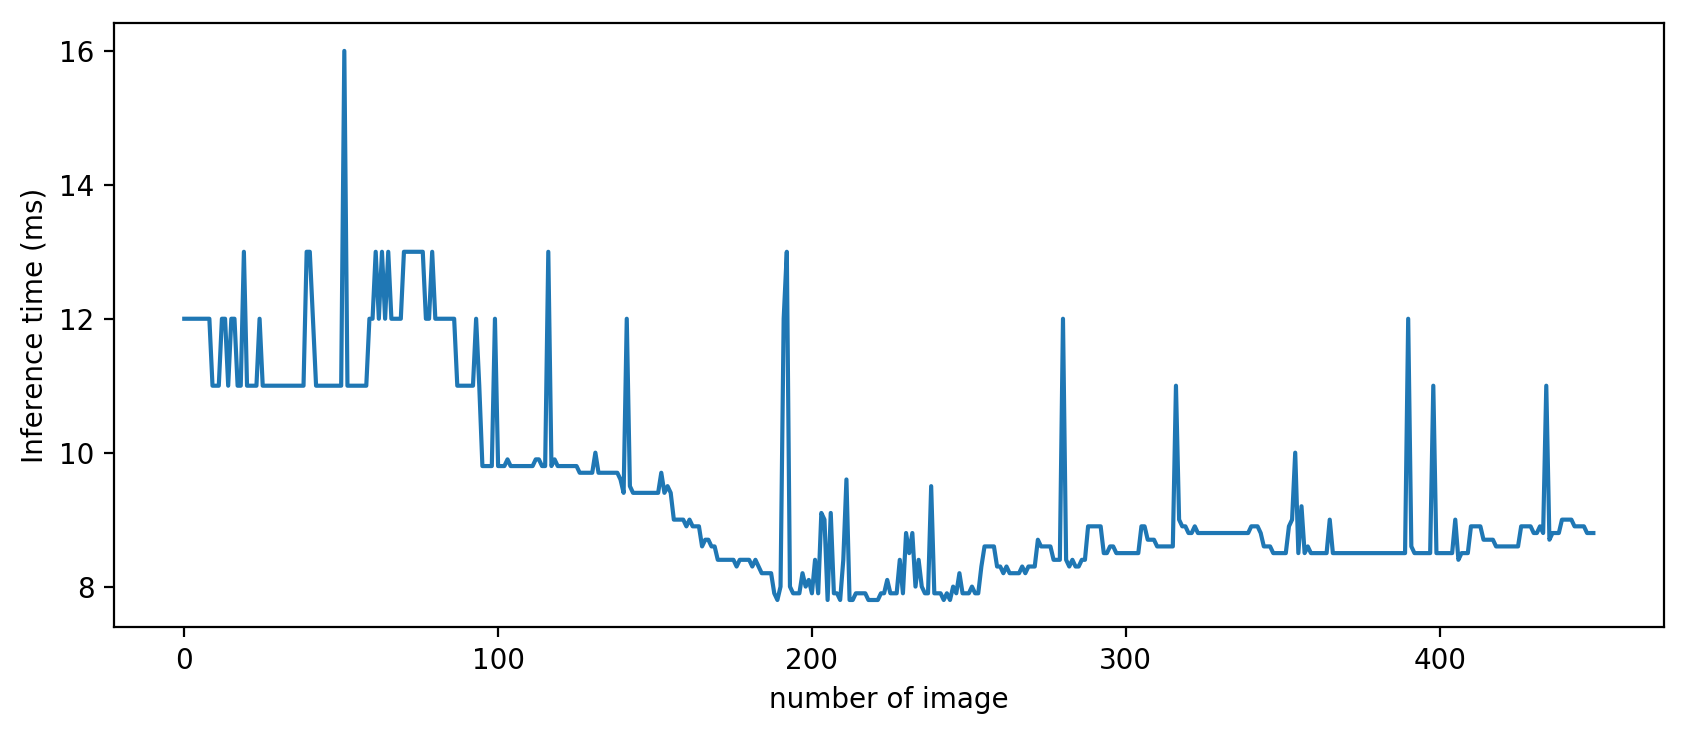
\includegraphics[width=15cm]{figures/Inftime_yolov5s_gpu.png}
    \caption{The inference time of YOLOv5s model, when it run on GPU}
    \label{fig: gpus}
\end{figure}
\begin{figure}[H]
    \centering
    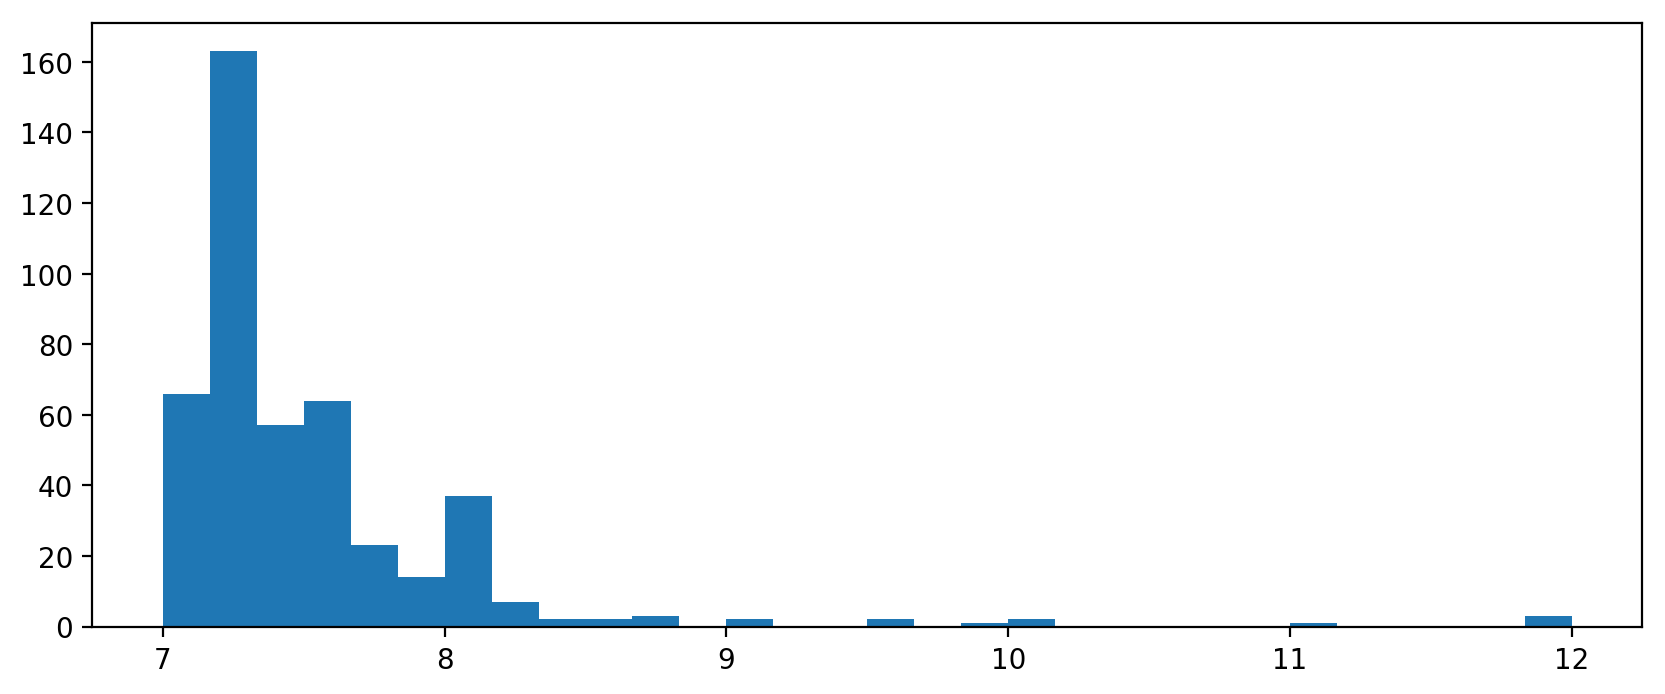
\includegraphics[width=15cm]{figures/Inftime_yolov5s_gpu_hist.png}
    \caption{The histogram of inference time of YOLOv5s model, when it run on GPU}
    \label{fig: gpus_hist}
\end{figure}
% \subsubsection*{GPU pro}
% Here the GPU model converted to the premium model. The inference time of YOLOv5s model on 470 images in test set of Kaggle data set is recorded and have been shown in Fig. \ref{fig: gpupro} and Fig. \ref{fig: gpupro_hist}.
% \begin{figure}[H]
%     \centering
%     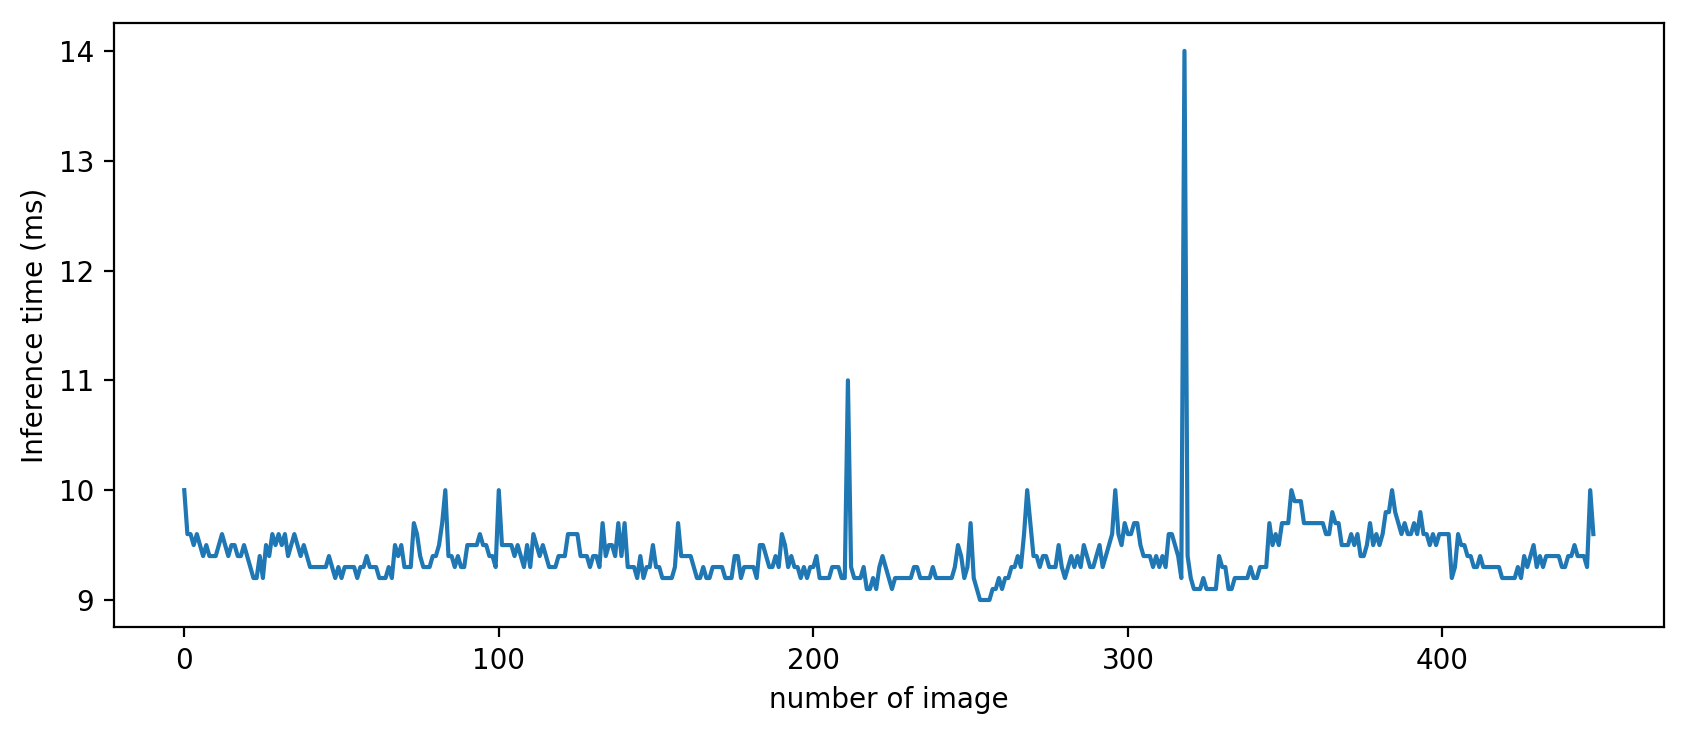
\includegraphics[width=15cm]{figures/gpupro.png}
%     \caption{The inference time of YOLOv5s model, when it run on premium GPU}
%     \label{fig: gpupro}
% \end{figure}
% \begin{figure}[H]
%     \centering
%     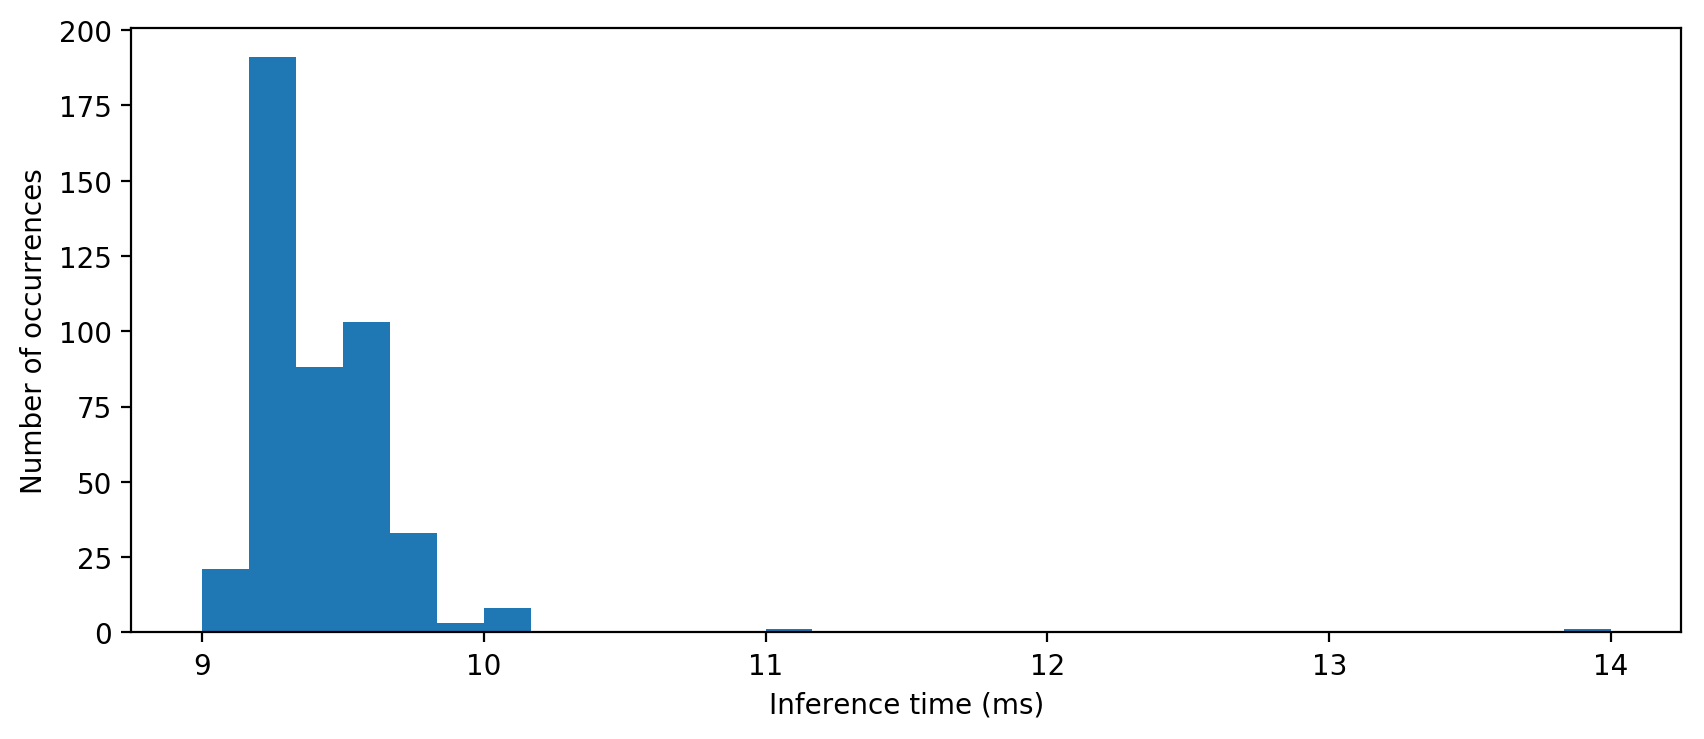
\includegraphics[width=15cm]{figures/gpupro_hist.png}
%     \caption{The histogram of inference time of YOLOv5s model, when it run on premium GPU}
%     \label{fig: gpupro_hist}
% \end{figure}
The maximum inference time is equal to 16.0(ms). The minimum inference time is 7.8 (ms) and the standard deviation is 1.42. The total time is 4.232 (s).

\subsection*{Half precision}
The inference time of YOLOv5s model with half precision on 470 images in test set of Kaggle data set is recorded and have been shown in Fig. \ref{fig: gpush} and Fig. \ref{fig: gpush_hist}.
\begin{figure}[H]
    \centering
    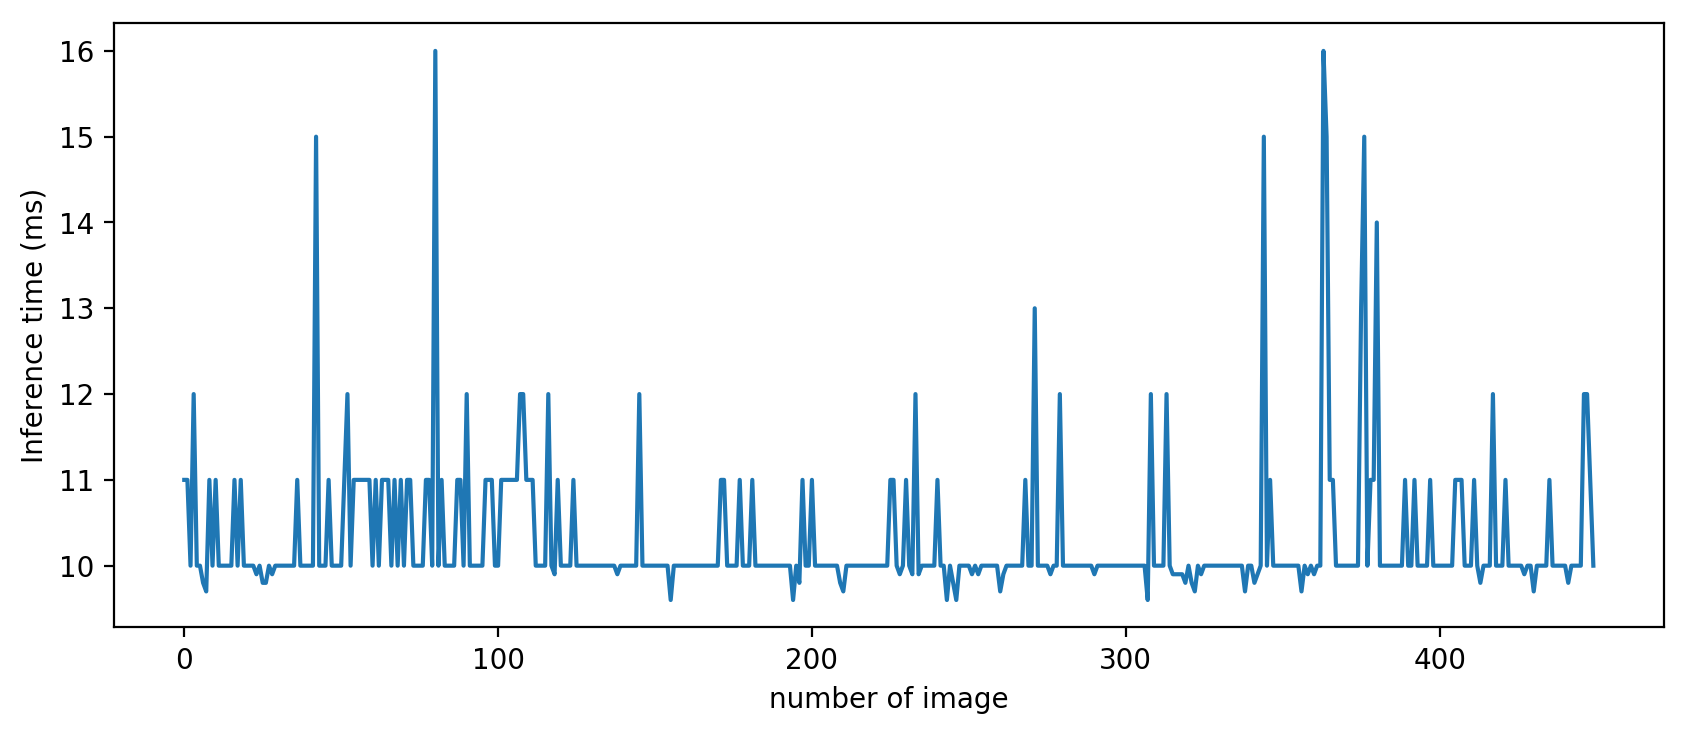
\includegraphics[width=15cm]{figures/Inftime_yolov5s_half.png}
    \caption{The inference time of YOLOv5s model, when it run on GPU with half precision}
    \label{fig: gpush}
\end{figure}
\begin{figure}[H]
    \centering
    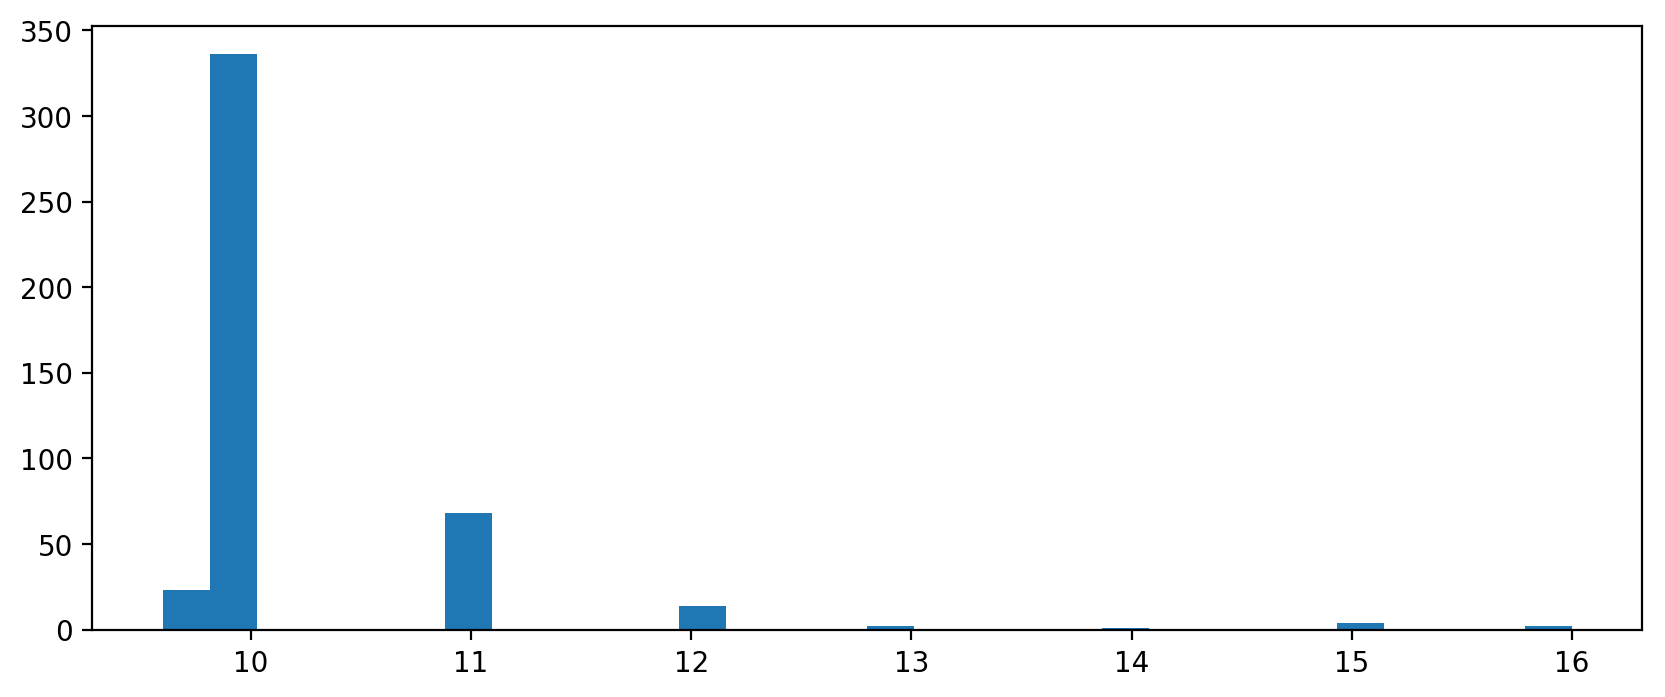
\includegraphics[width=15cm]{figures/Inftime_yolov5s_half_hist.png}
    \caption{The histogram of inference time of YOLOv5s model, when it run on GPU with half precision}
    \label{fig: gpush_hist}
\end{figure}
% Here the inference time of Yolov5s model on 470 images of kaggle data set, with half precision is shown in Fig. \ref{fig: gpus_half}. Fig. \ref{fig: gpus_half_hist} shows the histogram of these recorded time.
% \begin{figure}[H]
%     \centering
%     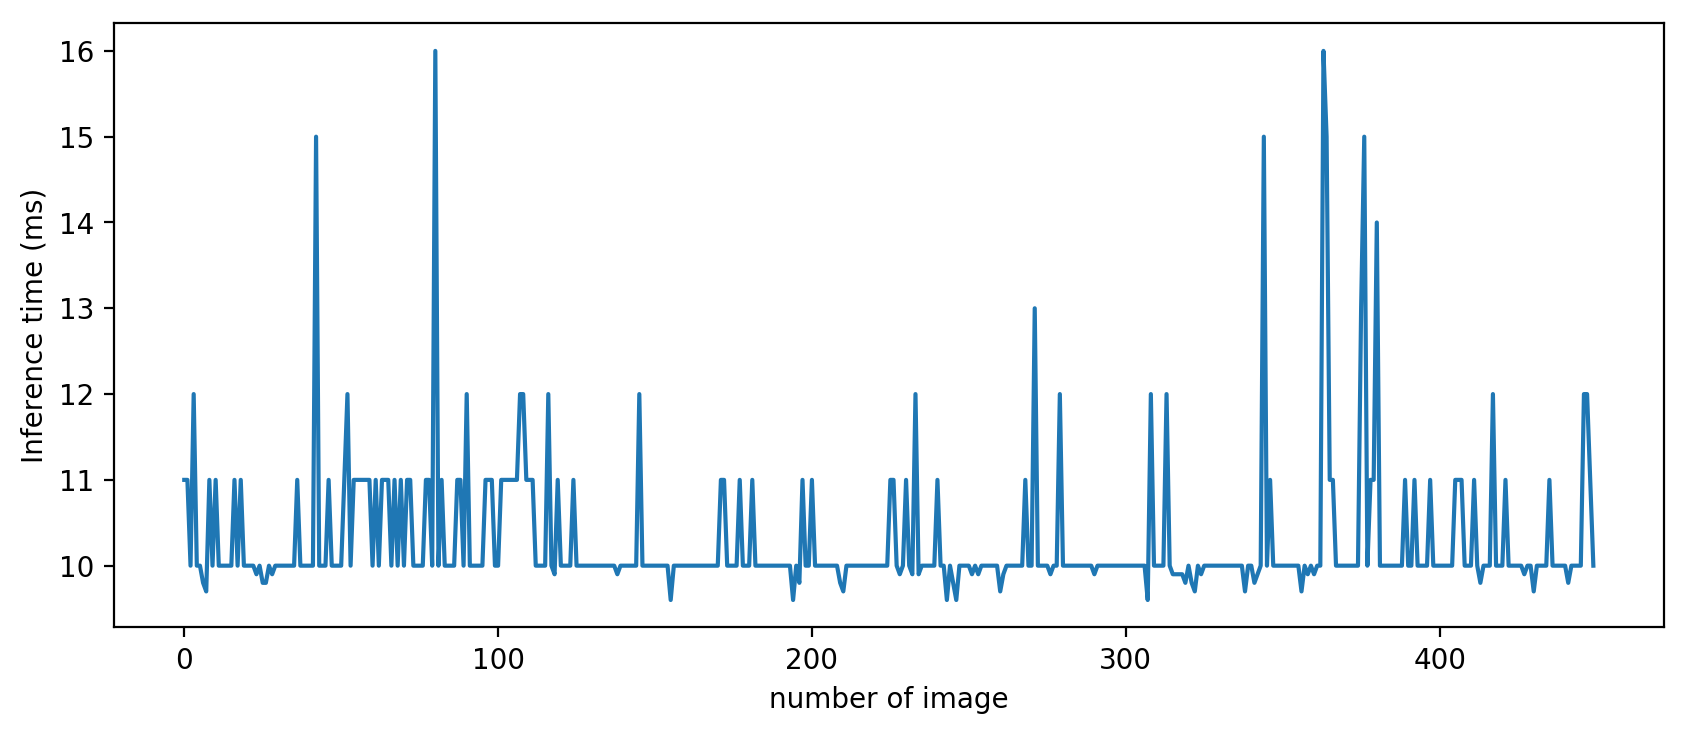
\includegraphics[width=15cm]{figures/Inftime_yolov5s_half.png}
%     \caption{The inference time of YOLOv5s model with half precision, when it run on GPU}
%     \label{fig: gpus_half}
% \end{figure}
% \begin{figure}[H]
%     \centering
%     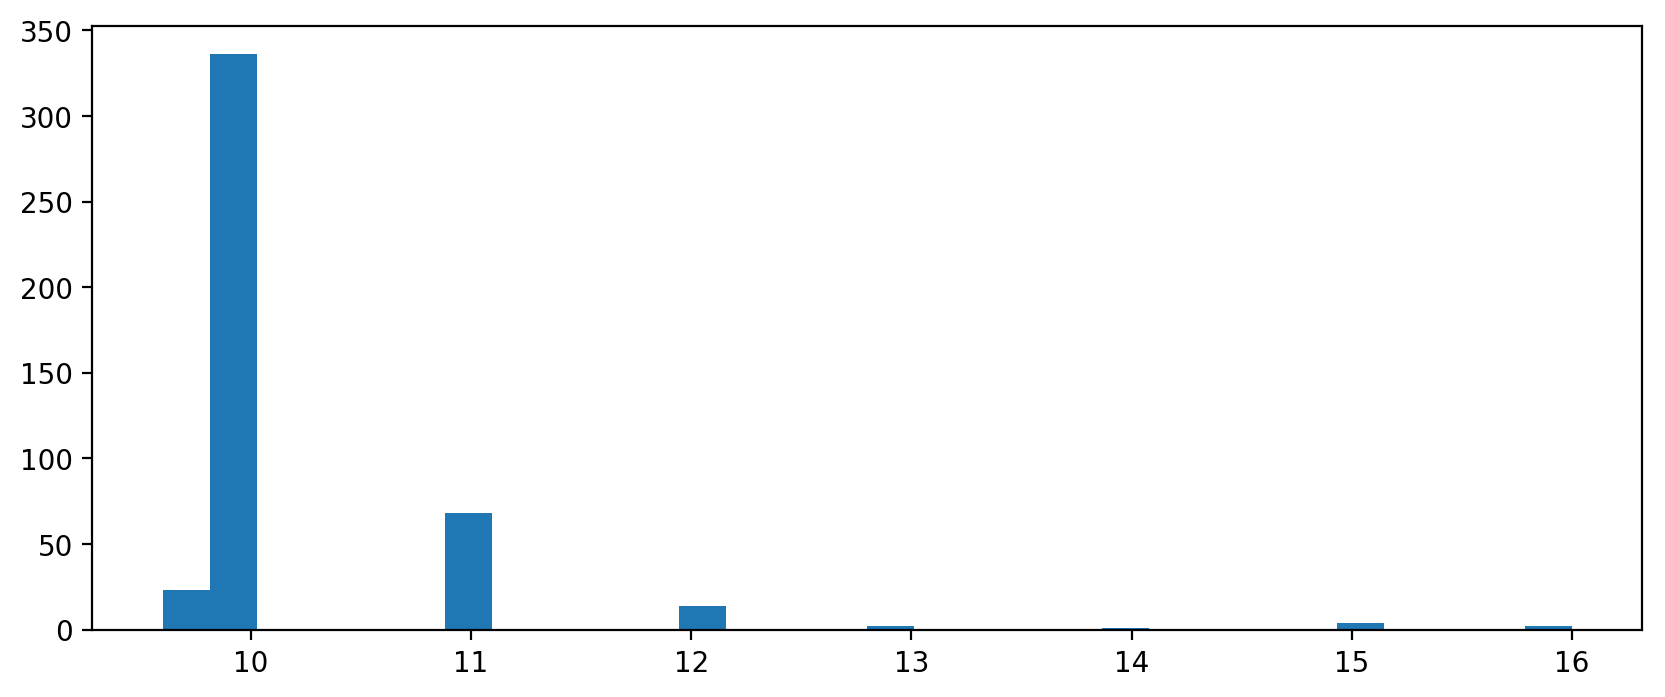
\includegraphics[width=15cm]{figures/Inftime_yolov5s_half_hist.png}
%     \caption{The histogram of inference time of YOLOv5s model with half precision, when it run on GPU}
%     \label{fig: gpus_half_hist}
% \end{figure}
% % \subsubsection*{GPU pro}
The maximum inference time is equal to 16.0 (ms). The minimum inference time is 9.6 (ms) and the standard deviation is 0.81. The total time is 4.629 (s).

%%%%%%%%%%%%%%% NEW SECTION %%%%%%%%%%%%%%%
\subsection*{Inference time of CPU}
Here you can find the inference time of Yolov5s model on 470 images of kaggle data set, which selected as a test set in Fig. \ref{fig: cpus}. Fig. \ref{fig: cpus_hist} shows the histogram of these time.
\begin{figure}[H]
    \centering
    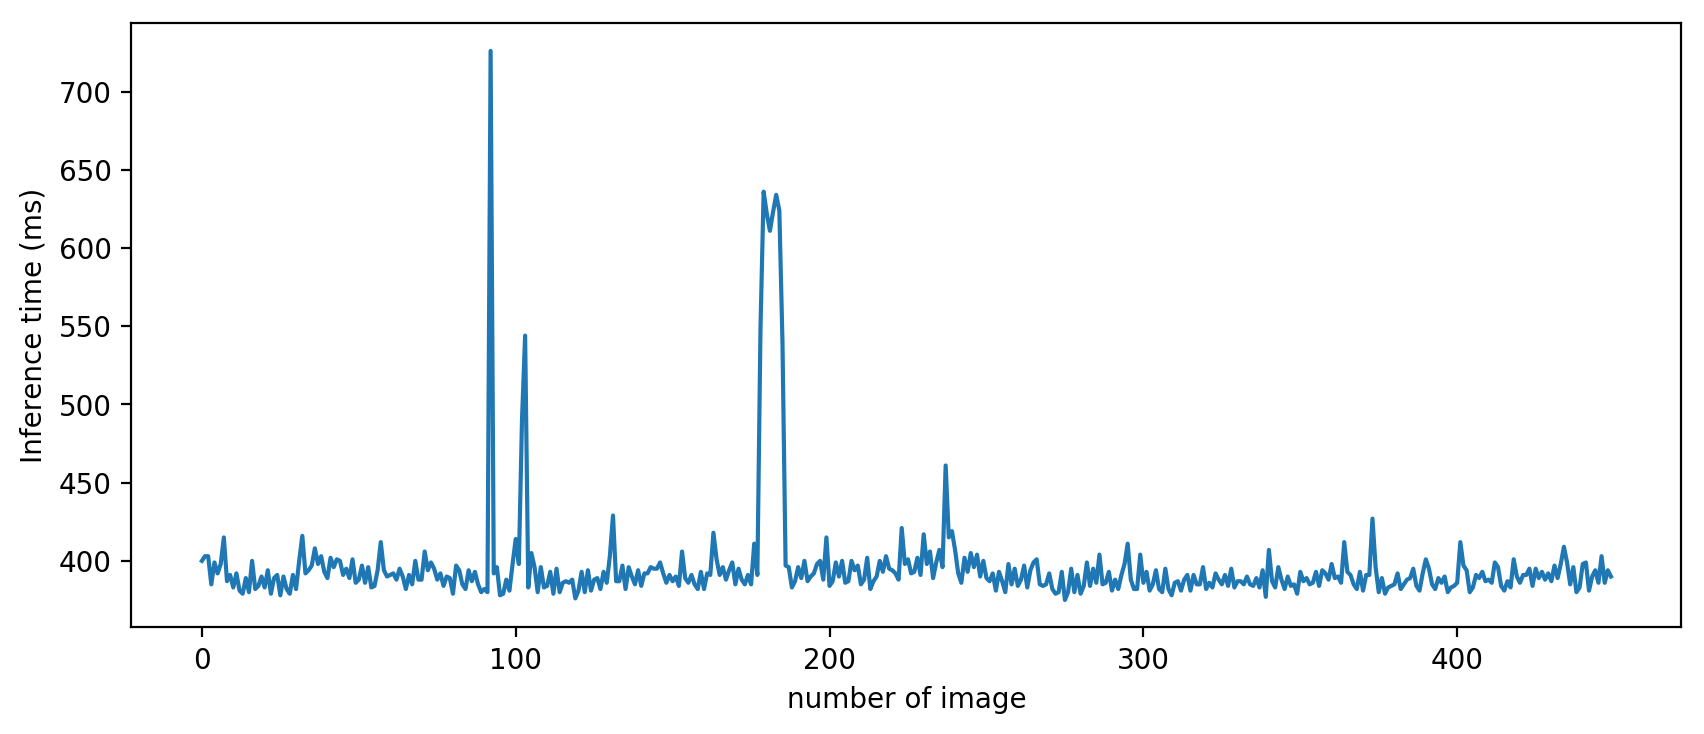
\includegraphics[width=15cm]{figures/Inftime_yolov5s_cpu.png}
    \caption{The inference time of YOLOv5s model, when it run on CPU}
    \label{fig: cpus}
\end{figure}
\begin{figure}[H]
    \centering
    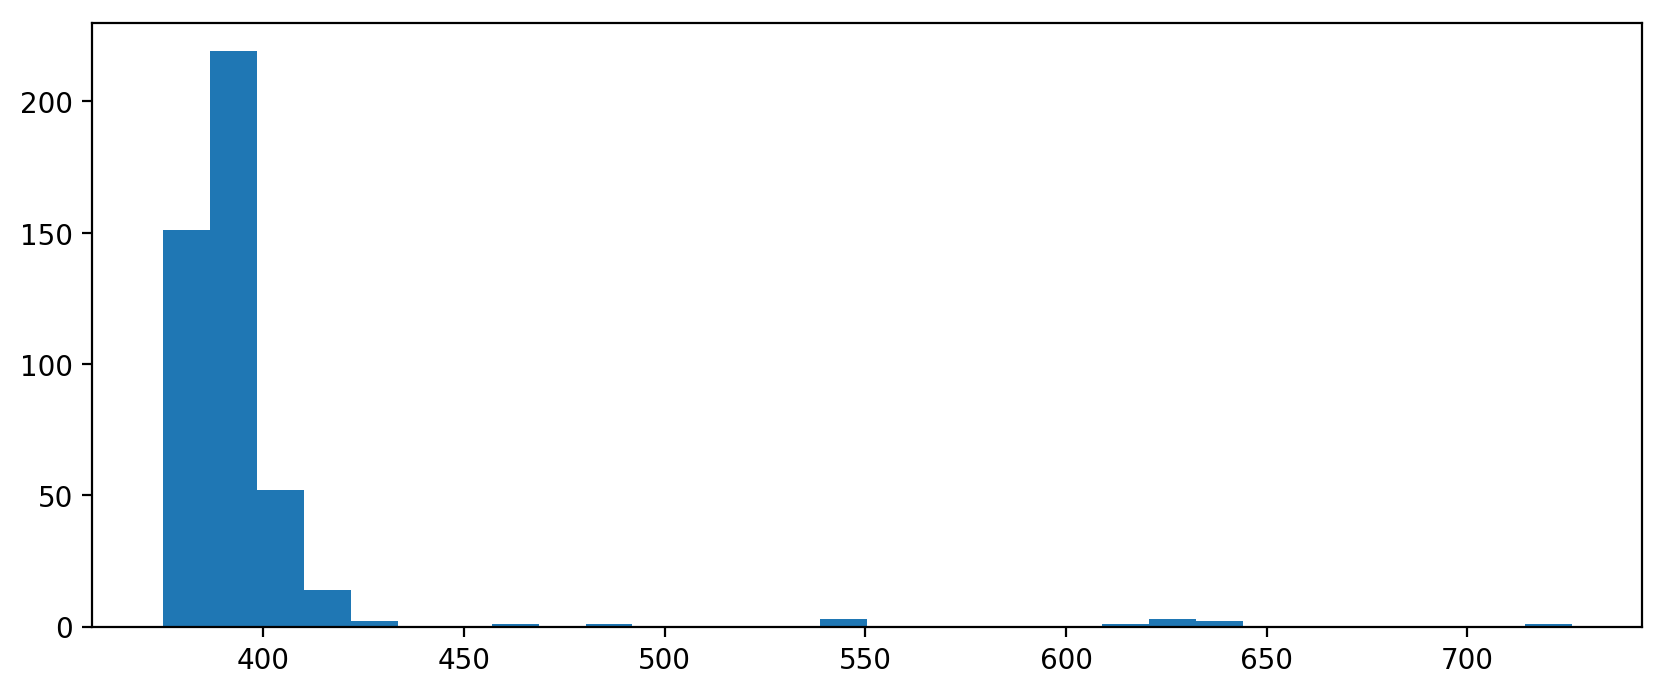
\includegraphics[width=15cm]{figures/Inftime_yolov5s_cpu_hist.png}
    \caption{The histogram of inference time of YOLOv5s model, when it run on CPU}
    \label{fig: cpus_hist}
\end{figure}
The maximum inference time is equal to 726.0 (ms). The minimum inference time is 375.0 (ms) and the standard deviation is 34.82. The total time is 178.255 (s).

\section*{YOLOv5 Medium}
\subsection*{Inference time of GPU}
 Here you can find the inference time of Yolov5m model on 470 images of kaggle data set, which selected as a test set in Fig. \ref{fig: gpum}. Fig. \ref{fig: gpum_hist} shows the histogram of these time.
\begin{figure}[H]
    \centering
    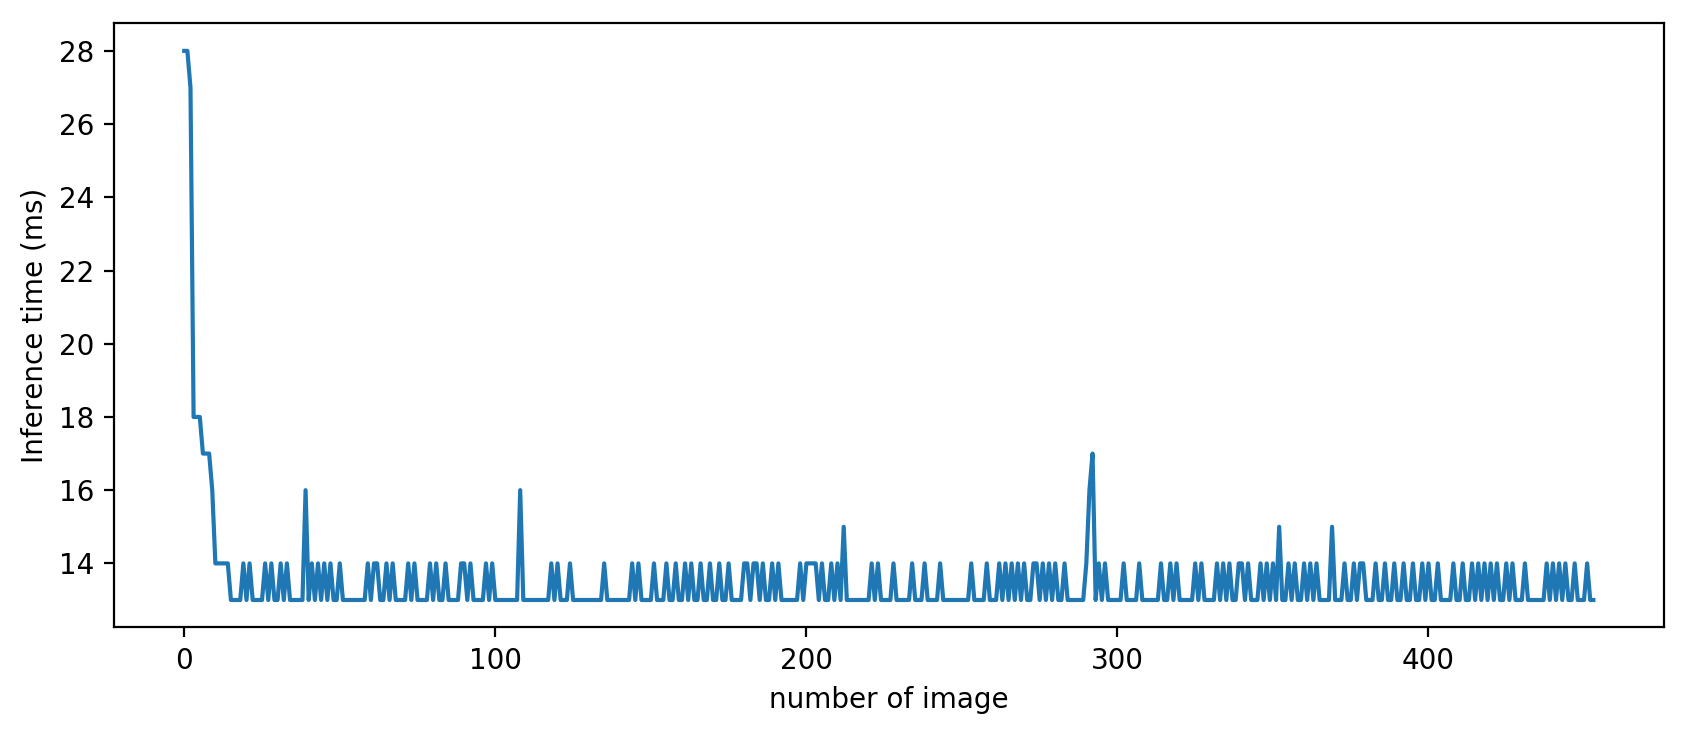
\includegraphics[width=15cm]{figures/Inftime_yolovM_gpu.png}
    \caption{The inference time of YOLOv5m model, when it run on GPU}
    \label{fig: gpum}
\end{figure}
\begin{figure}[H]
    \centering
    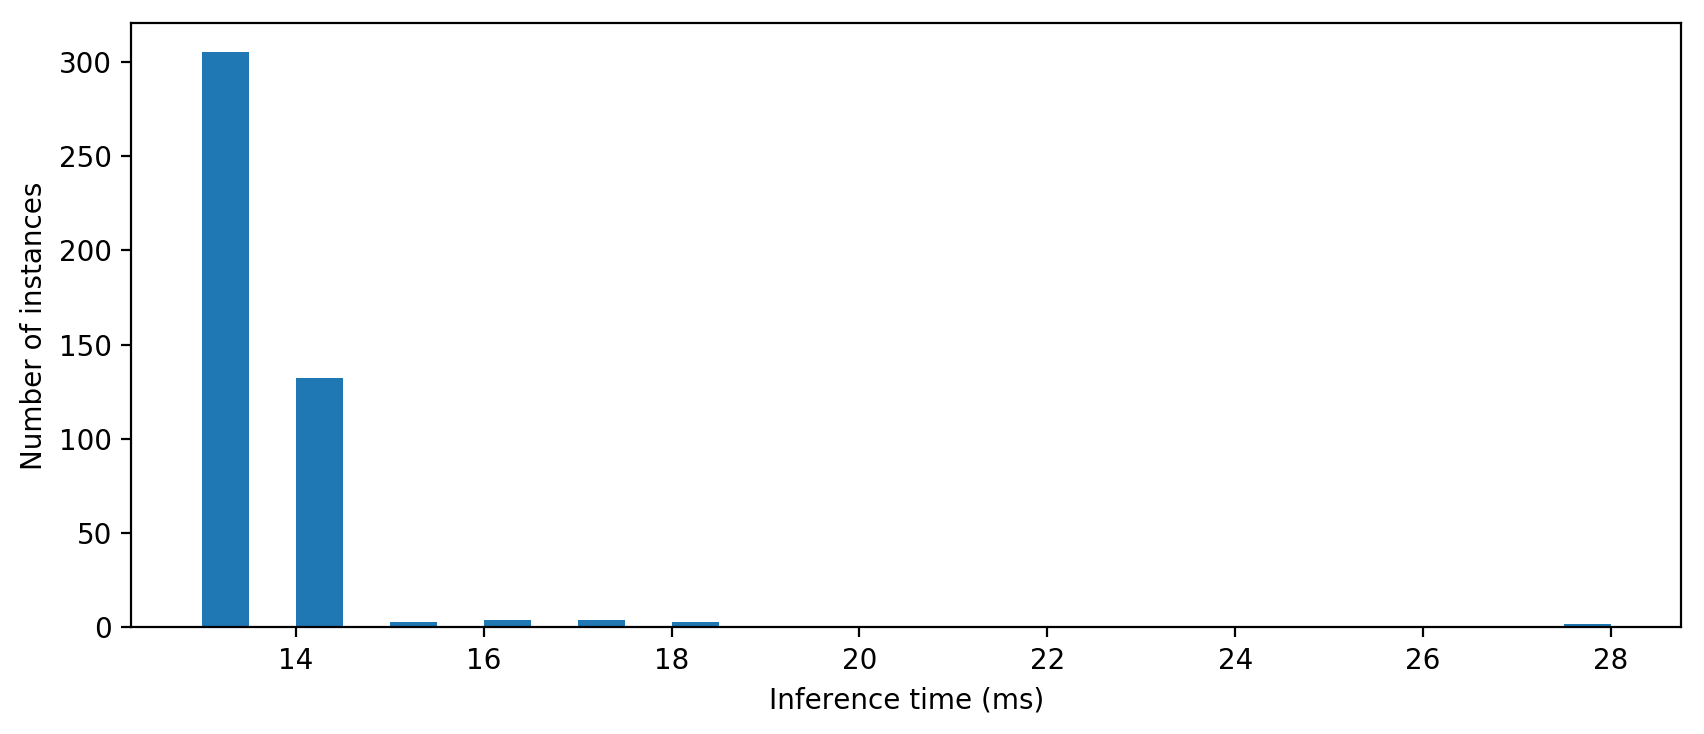
\includegraphics[width=15cm]{figures/Inftime_yolov5M_gpu_hist.png}
    \caption{The histogram of inference time of YOLOv5m model, when it run on GPU}
    \label{fig: gpum_hist}
\end{figure}
% \subsubsection*{GPU pro}
% Here the GPU model converted to the premium model. The inference time of YOLOv5s model on 470 images in test set of Kaggle data set is recorded and have been shown in Fig. \ref{fig: gpupro} and Fig. \ref{fig: gpupro_hist}.
% \begin{figure}[H]
%     \centering
%     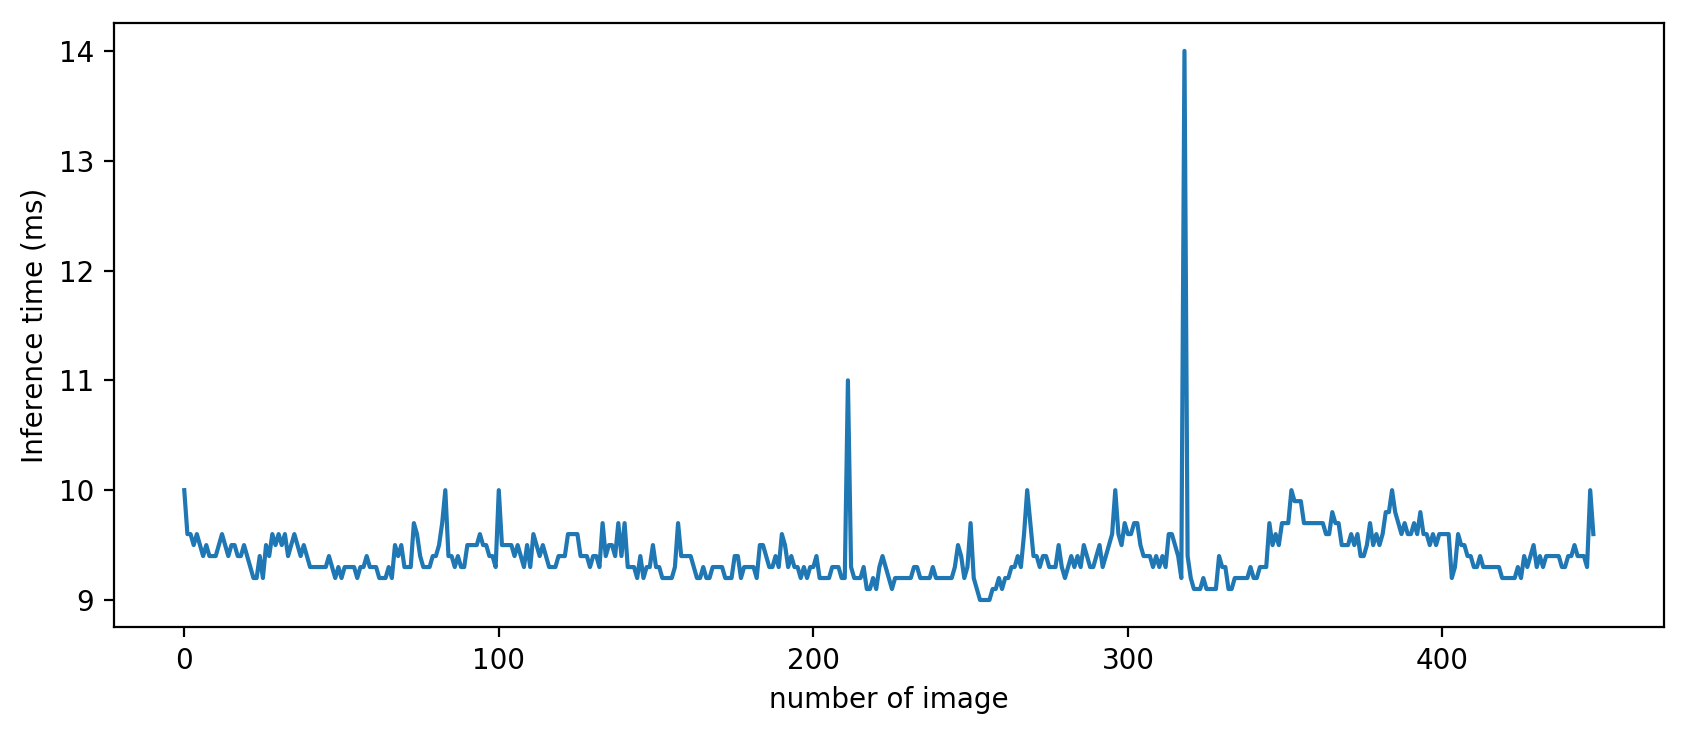
\includegraphics[width=15cm]{figures/gpupro.png}
%     \caption{The inference time of YOLOv5s model, when it run on premium GPU}
%     \label{fig: gpupro}
% \end{figure}
% \begin{figure}[H]
%     \centering
%     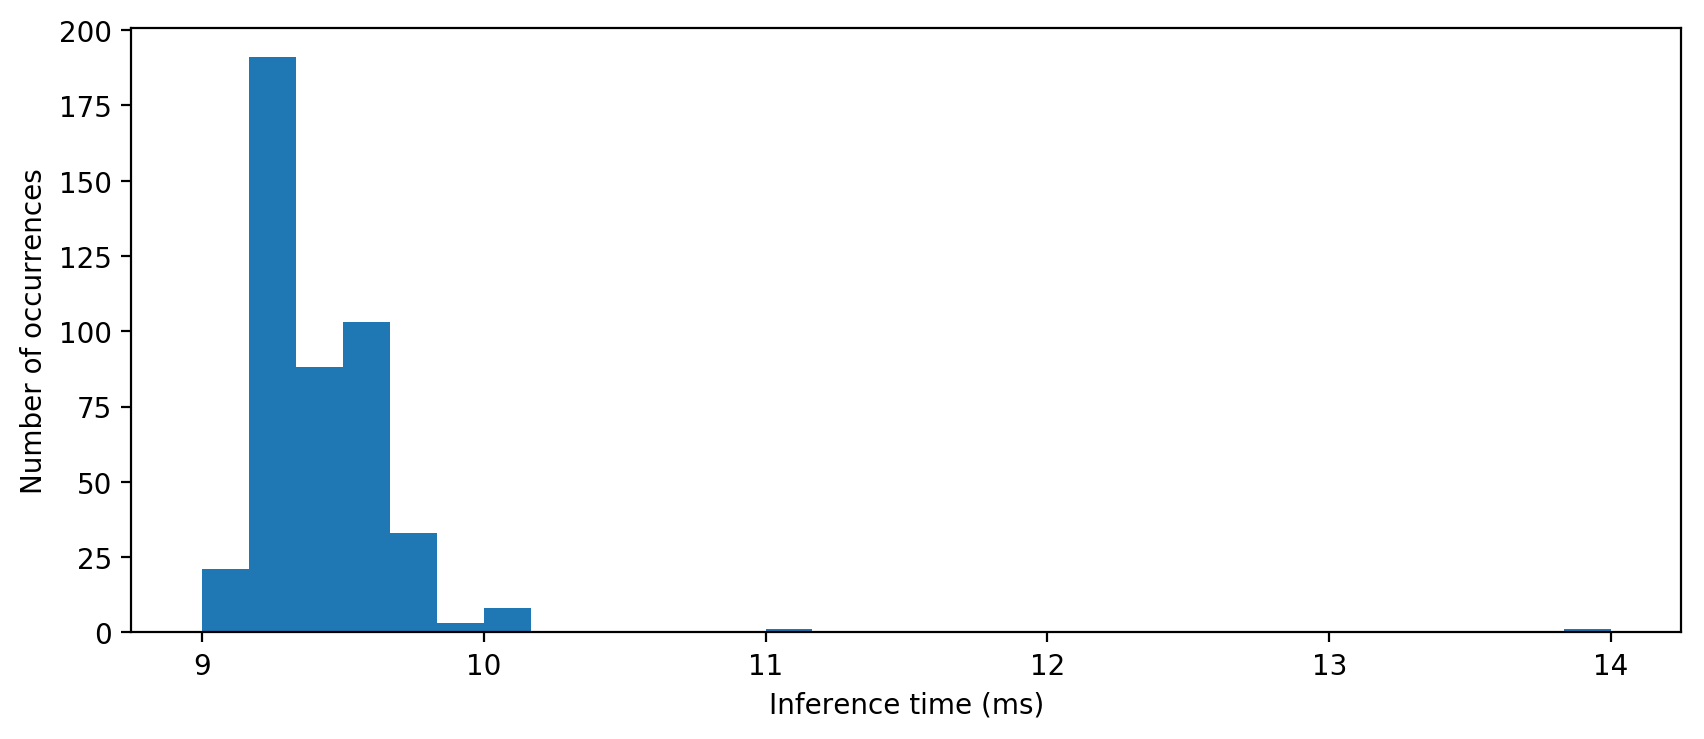
\includegraphics[width=15cm]{figures/gpupro_hist.png}
%     \caption{The histogram of inference time of YOLOv5s model, when it run on premium GPU}
%     \label{fig: gpupro_hist}
% \end{figure}
The maximum inference time is equal to 28.0 (ms). The minimum inference time is 13.0 (ms) and the standard deviation is 1.37. The total time is 6.127 (s).

\subsection*{Half precision}
The inference time of YOLOv5m model with half precision on 470 images in test set of Kaggle data set is recorded and have been shown in Fig. \ref{fig: gpumh} and Fig. \ref{fig: gpumh_hist}.
\begin{figure}[H]
    \centering
    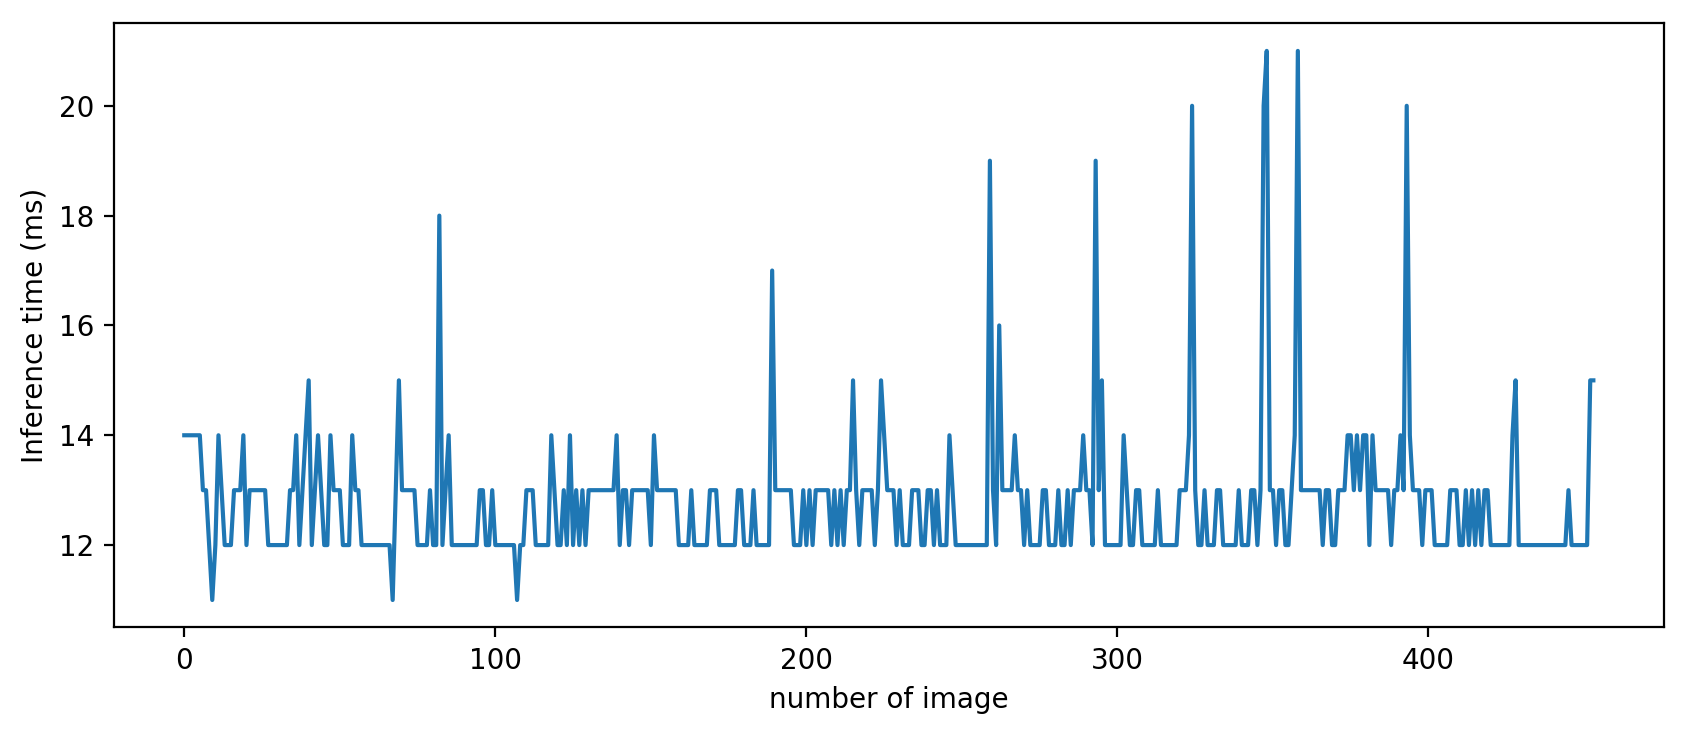
\includegraphics[width=15cm]{figures/Inftime_yolov5M_half.png}
    \caption{The inference time of YOLOv5m model, when it run on GPU with half precision}
    \label{fig: gpumh}
\end{figure}
\begin{figure}[H]
    \centering
    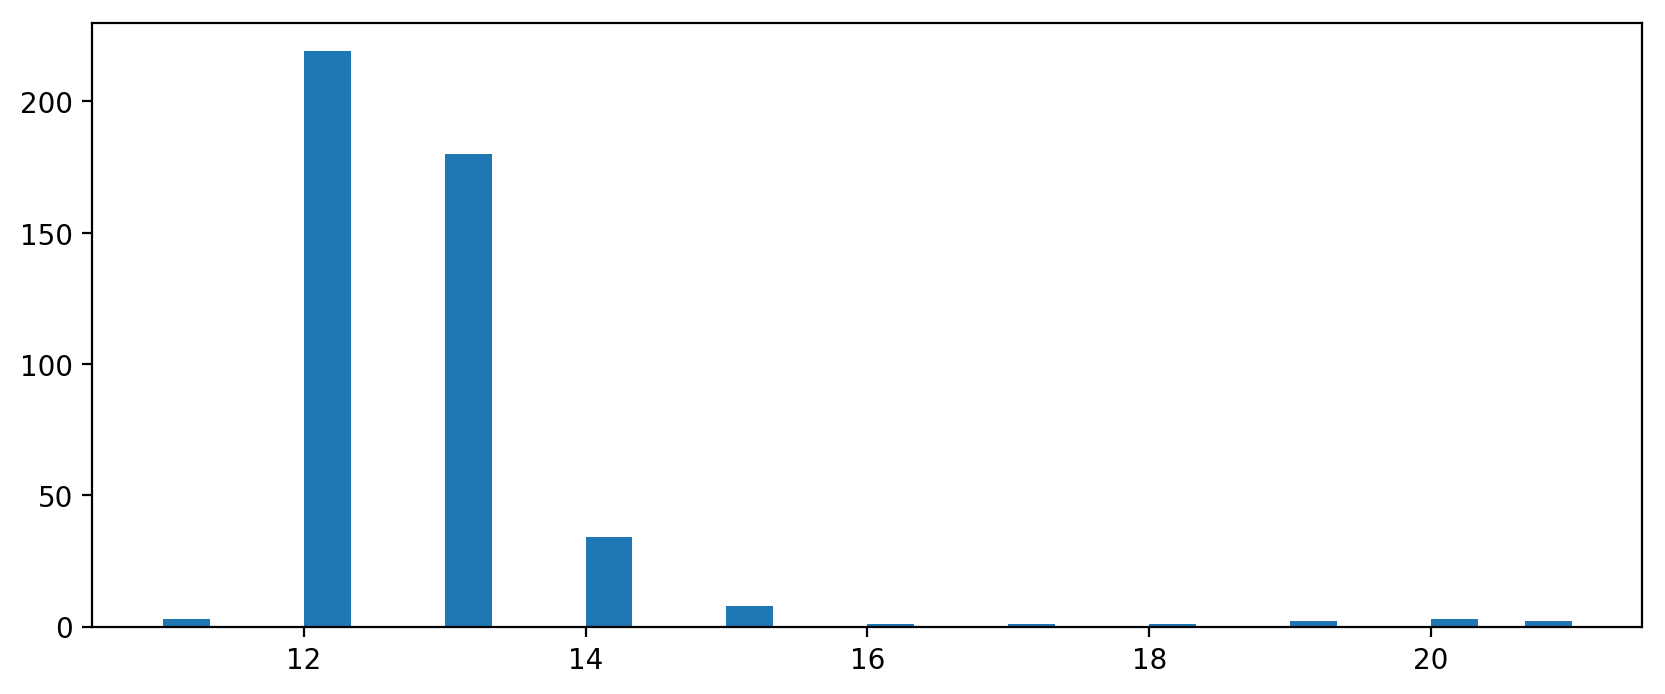
\includegraphics[width=15cm]{figures/Inftime_yolov5M_half_hist.png}
    \caption{The histogram of inference time of YOLOv5m model, when it run on GPU with half precision}
    \label{fig: gpumh_hist}
\end{figure}
% Here the inference time of Yolov5s model on 470 images of kaggle data set, with half precision is shown in Fig. \ref{fig: gpus_half}. Fig. \ref{fig: gpus_half_hist} shows the histogram of these recorded time.
% \begin{figure}[H]
%     \centering
%     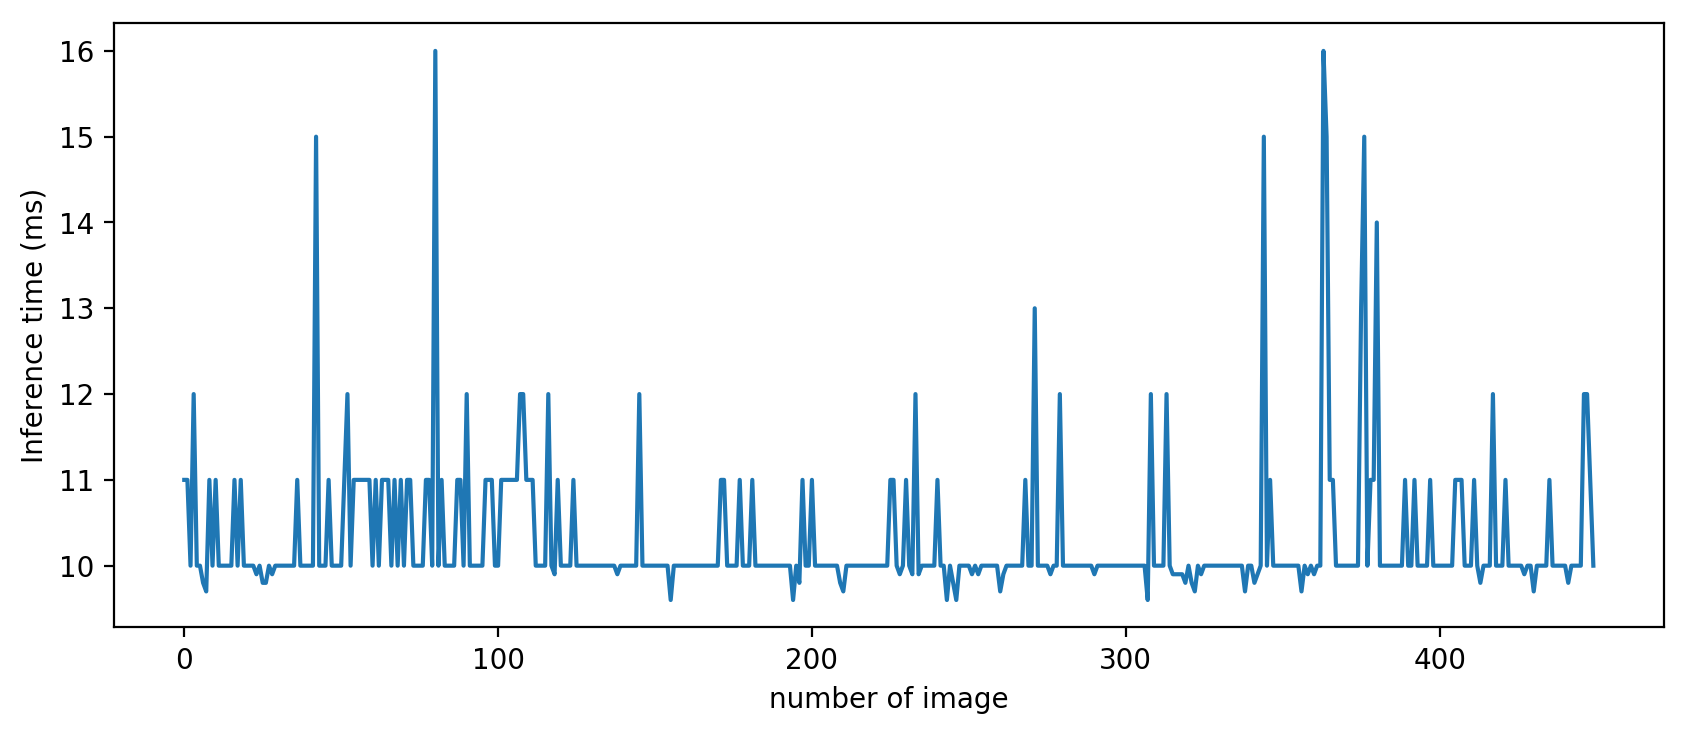
\includegraphics[width=15cm]{figures/Inftime_yolov5s_half.png}
%     \caption{The inference time of YOLOv5s model with half precision, when it run on GPU}
%     \label{fig: gpus_half}
% \end{figure}
% \begin{figure}[H]
%     \centering
%     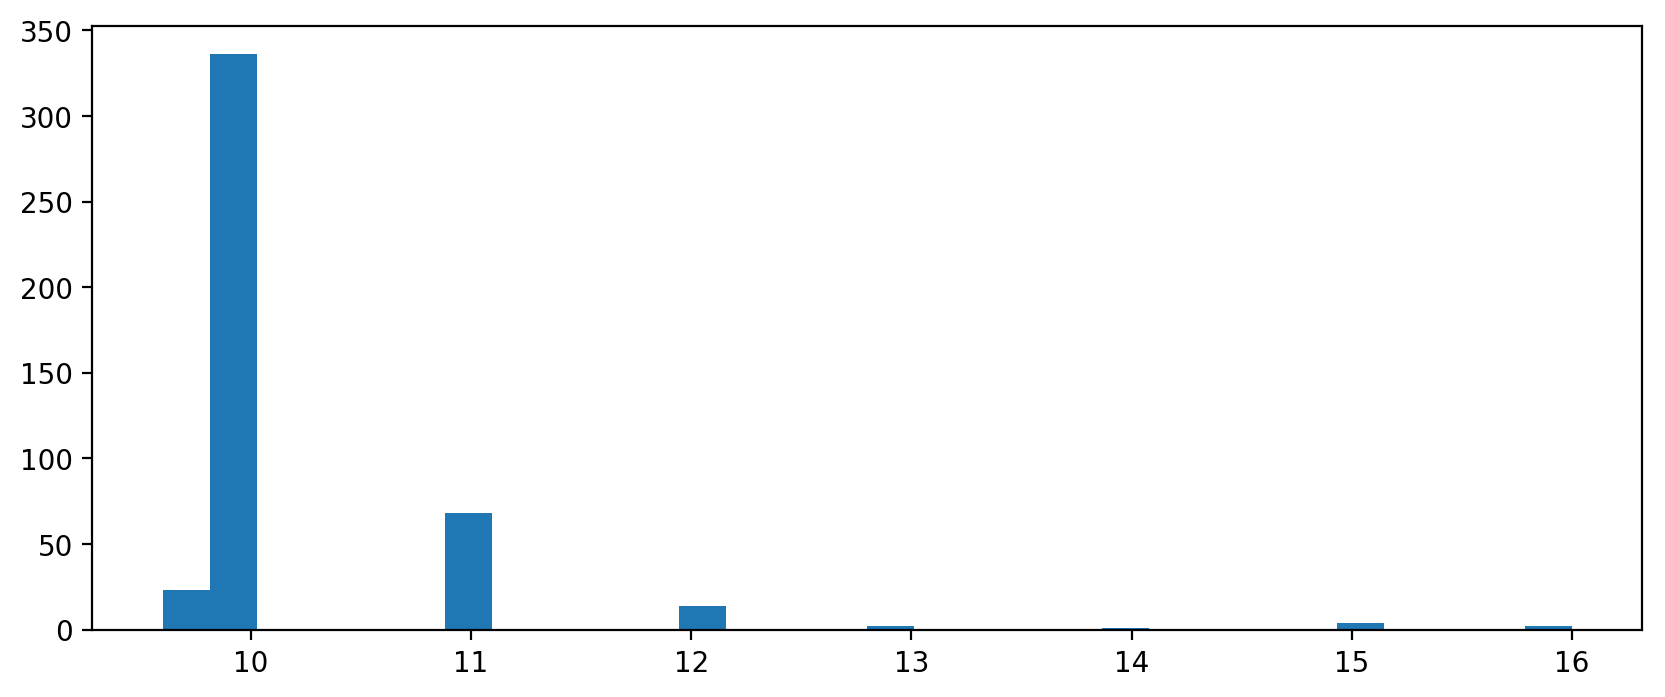
\includegraphics[width=15cm]{figures/Inftime_yolov5s_half_hist.png}
%     \caption{The histogram of inference time of YOLOv5s model with half precision, when it run on GPU}
%     \label{fig: gpus_half_hist}
% \end{figure}
% % \subsubsection*{GPU pro}
The maximum inference time is equal to 21.0 (ms). The minimum inference time is 11.0 (ms) and the standard deviation is 1.21. The total time is 5.788 (s).

%%%%%%%%%%%%%%% NEW SECTION %%%%%%%%%%%%%%%
\section*{Inference time of CPU}
Here you can find the inference time of Yolov5s model on 470 images of kaggle data set, which selected as a test set in Fig. \ref{fig: cpum}. Fig. \ref{fig: cpum_hist} shows the histogram of these time.
\begin{figure}[H]
    \centering
    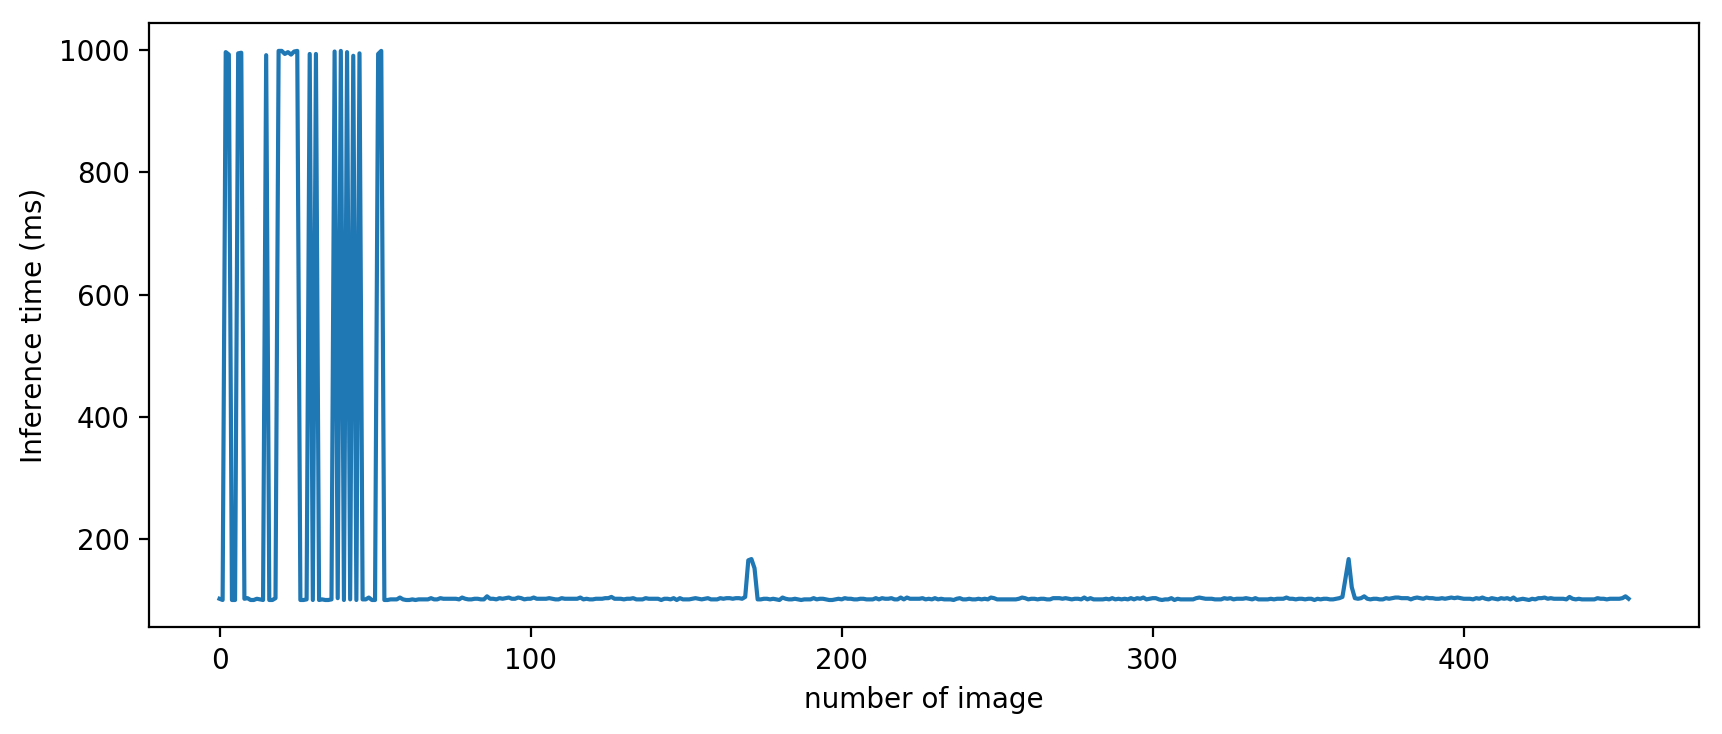
\includegraphics[width=15cm]{figures/Inftime_yolov5M_cpu.png}
    \caption{The inference time of YOLOv5s model, when it run on CPU}
    \label{fig: cpum}
\end{figure}
\begin{figure}[H]
    \centering
    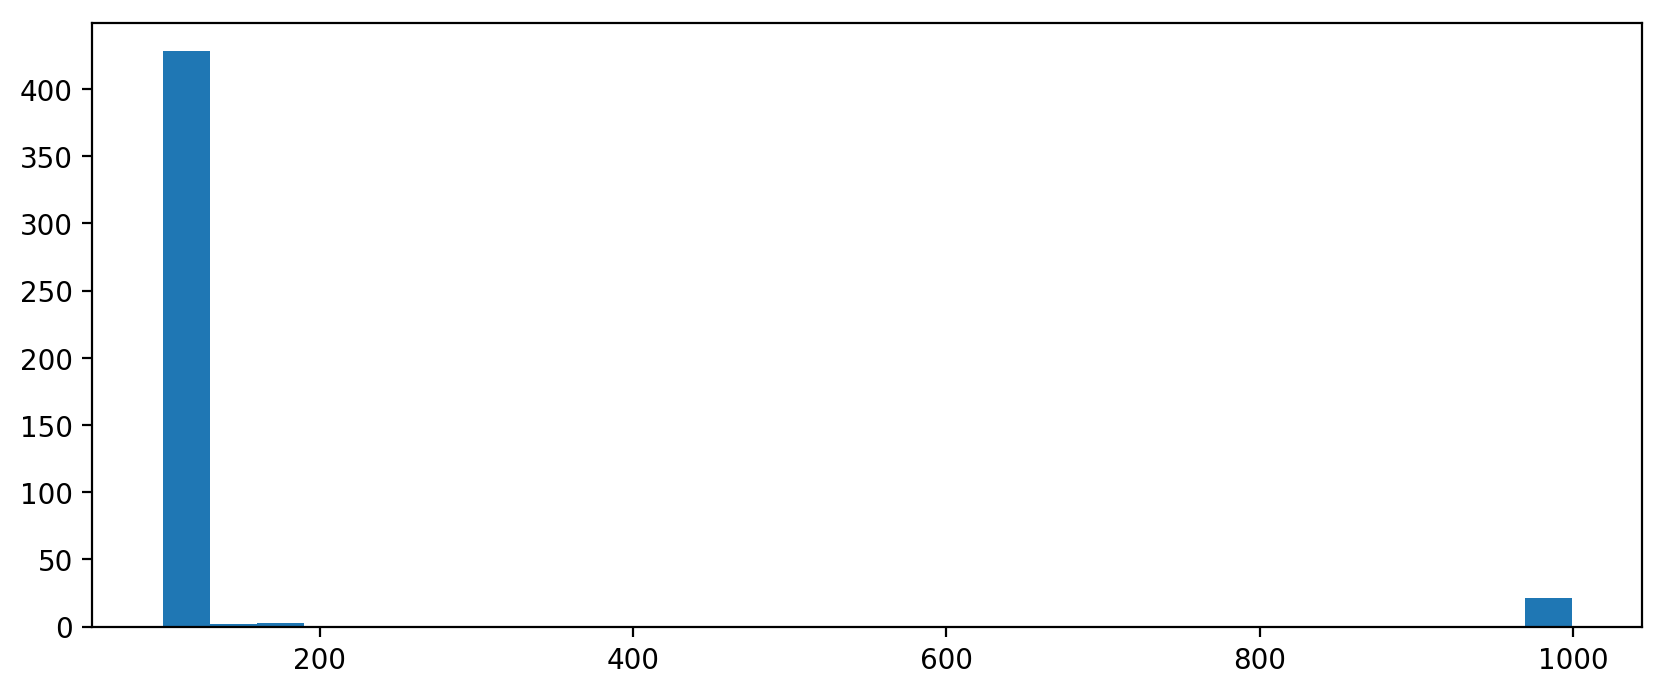
\includegraphics[width=15cm]{figures/Inftime_yolov5M_cpu_hist.png}
    \caption{The histogram of inference time of YOLOv5m model, when it run on CPU}
    \label{fig: cpum_hist}
\end{figure}
The maximum inference time is equal to 999.0 (ms). The minimum inference time is 100.0 (ms) and the standard deviation is 187.73. The total time is 65.311 (s).

\section*{YOLOv5 large}
\subsection*{Inference time of GPU}
 Here you can find the inference time of Yolov5l model on 470 images of kaggle data set, which selected as a test set in Fig. \ref{fig: gpul}. Fig. \ref{fig: gpul_hist} shows the histogram of these time.
\begin{figure}[H]
    \centering
    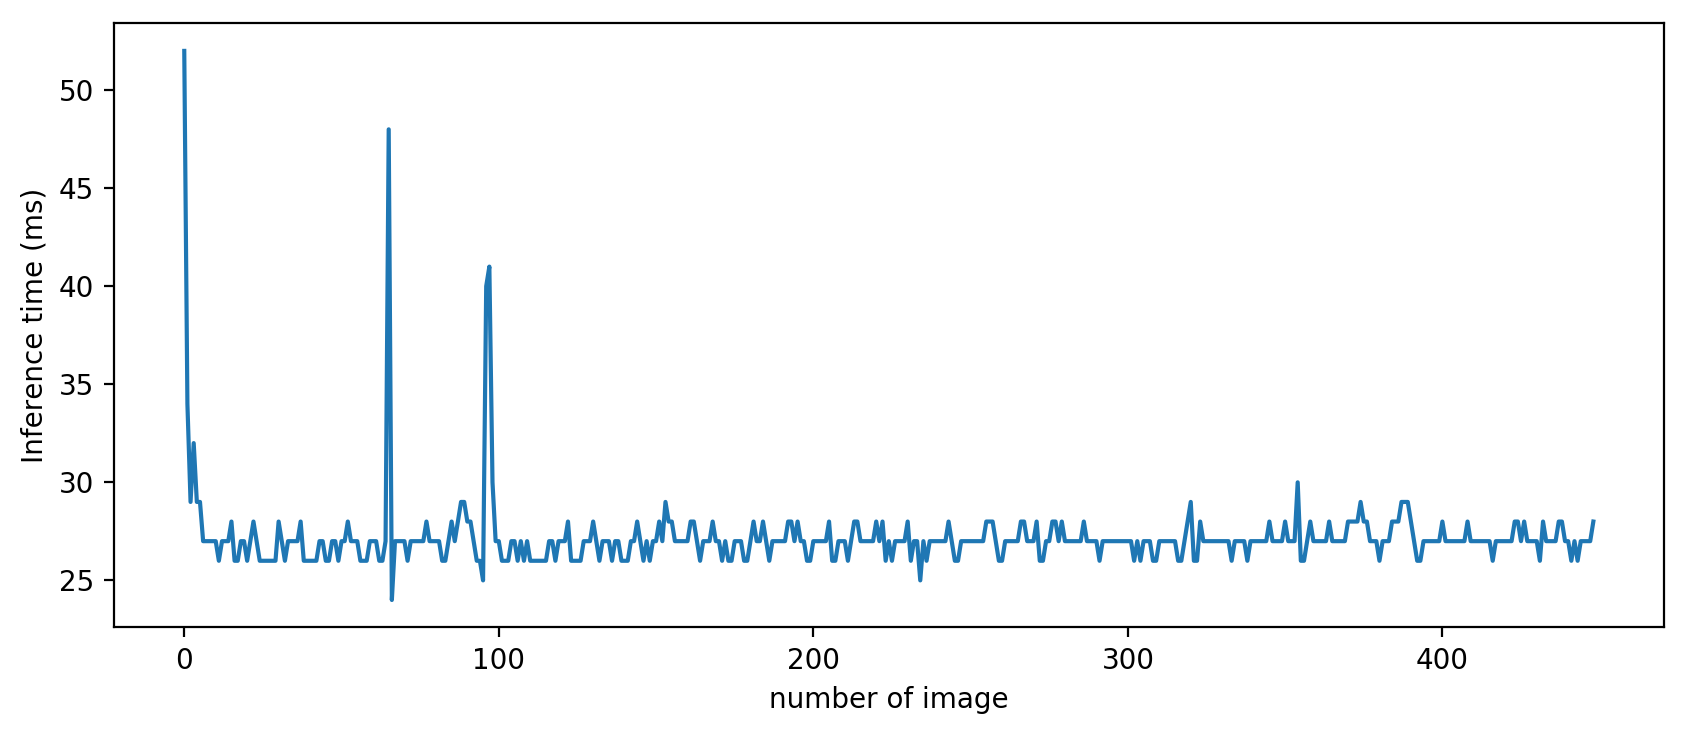
\includegraphics[width=15cm]{figures/Inftime_yolovL_gpu.png}
    \caption{The inference time of YOLOv5l model, when it run on GPU}
    \label{fig: gpul}
\end{figure}
\begin{figure}[H]
    \centering
    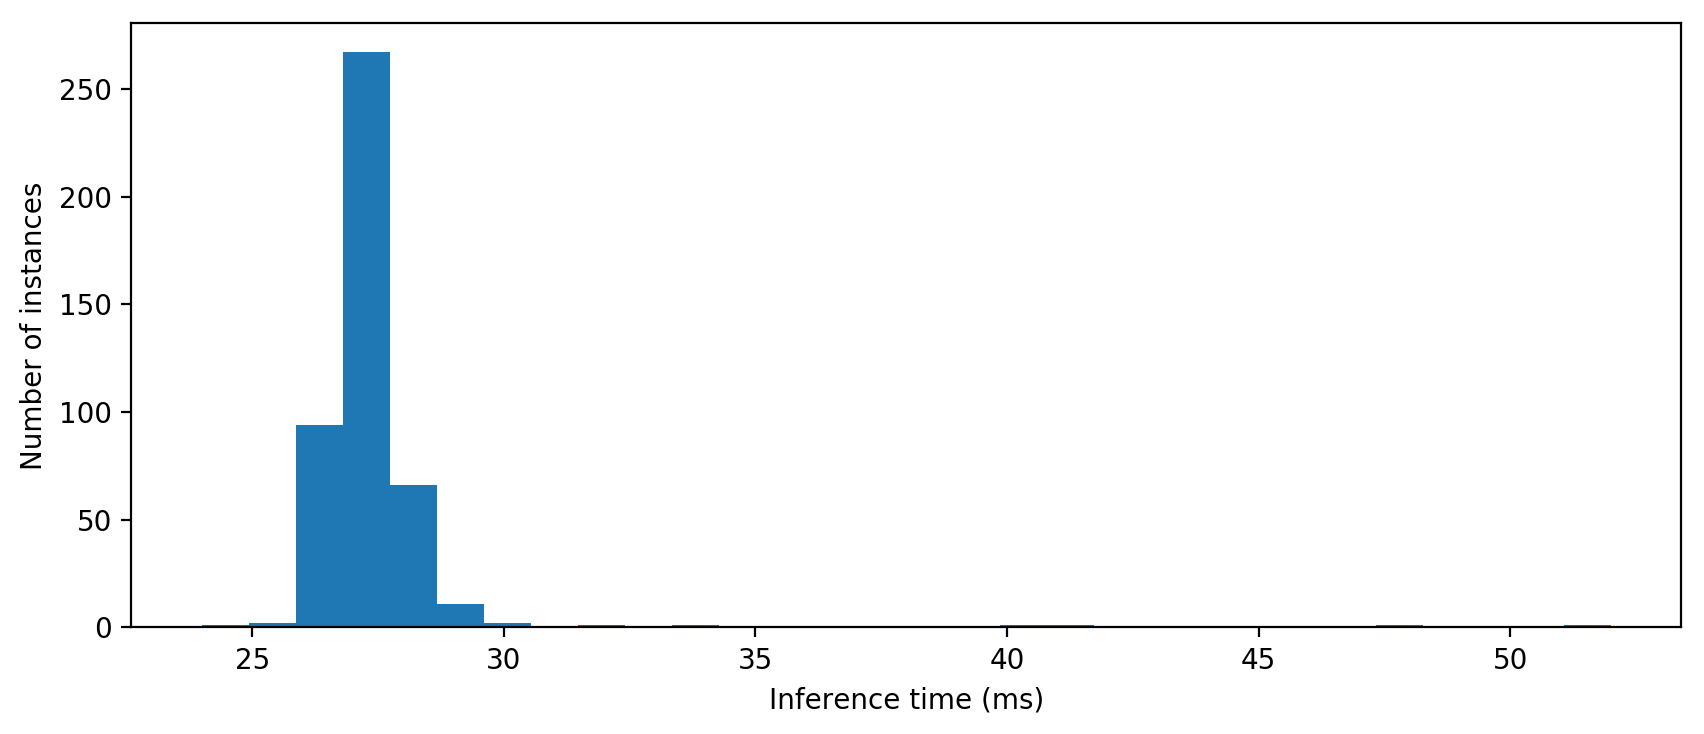
\includegraphics[width=15cm]{figures/Inftime_yolov5L_gpu_hist.png}
    \caption{The histogram of inference time of YOLOv5l model, when it run on GPU}
    \label{fig: gpul_hist}
\end{figure}
% \subsubsection*{GPU pro}
% Here the GPU model converted to the premium model. The inference time of YOLOv5s model on 470 images in test set of Kaggle data set is recorded and have been shown in Fig. \ref{fig: gpupro} and Fig. \ref{fig: gpupro_hist}.
% \begin{figure}[H]
%     \centering
%     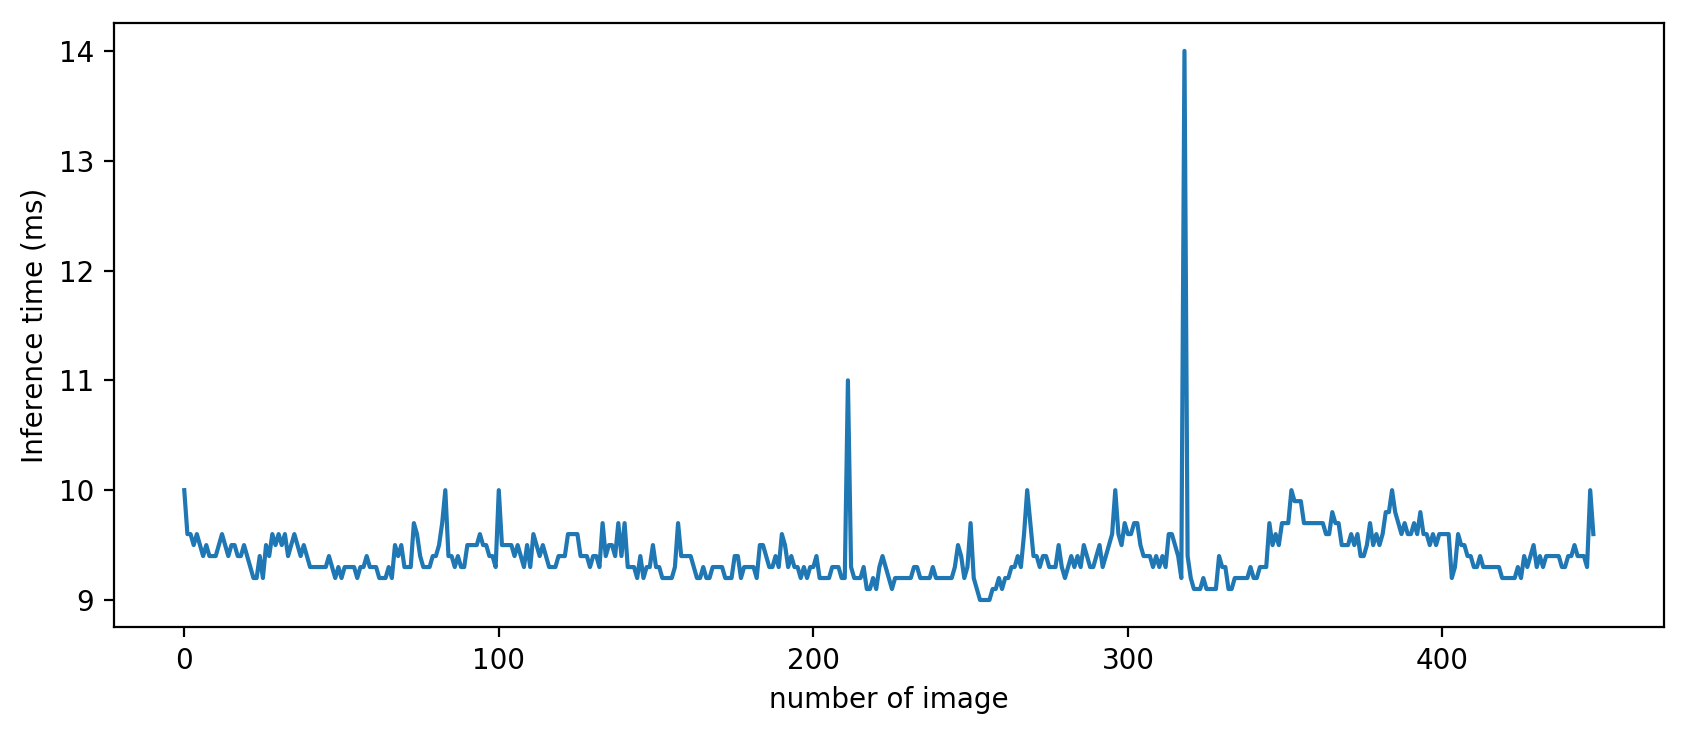
\includegraphics[width=15cm]{figures/gpupro.png}
%     \caption{The inference time of YOLOv5s model, when it run on premium GPU}
%     \label{fig: gpupro}
% \end{figure}
% \begin{figure}[H]
%     \centering
%     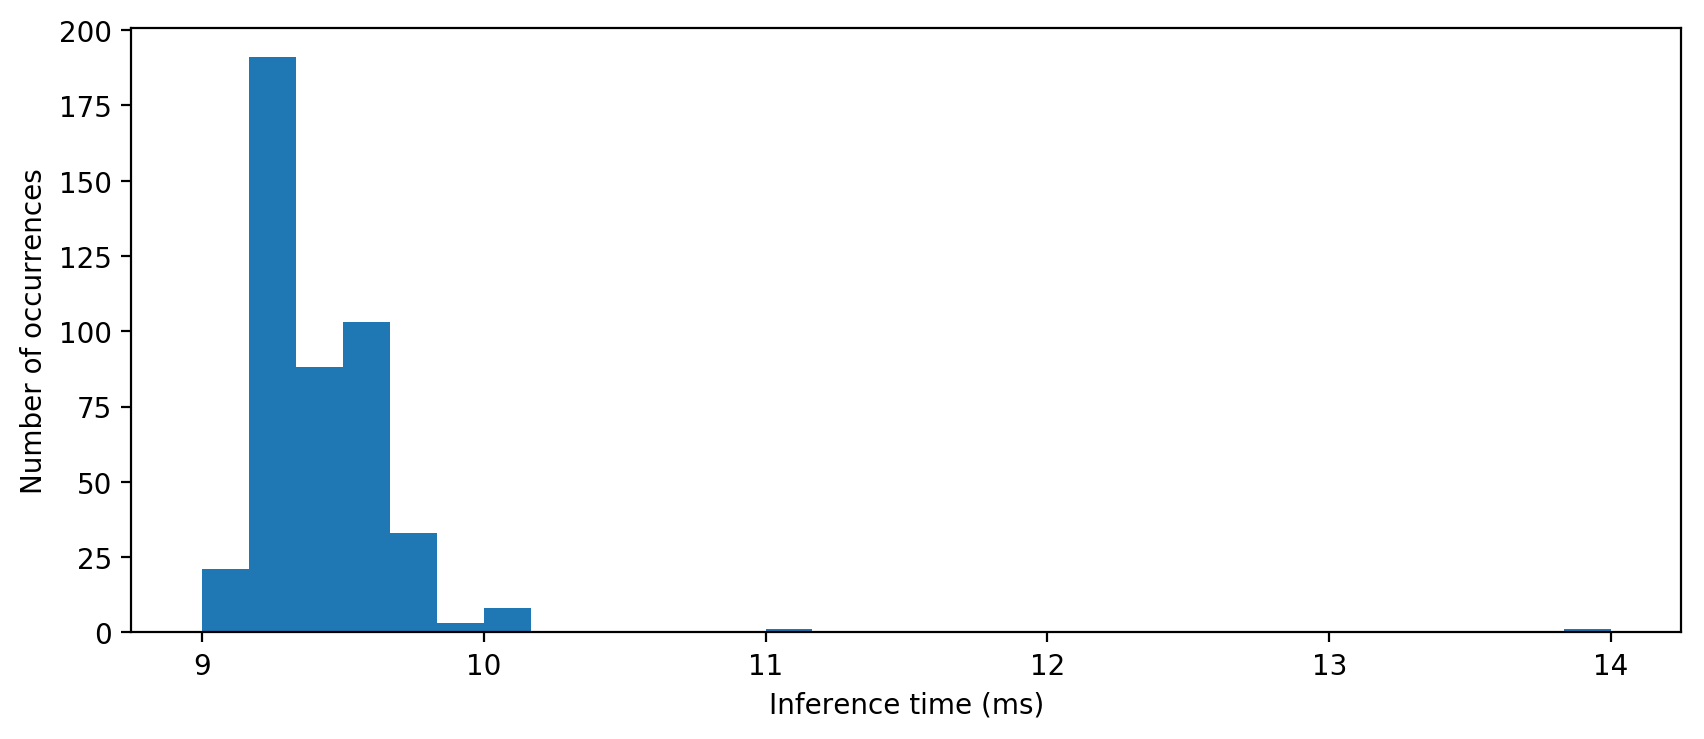
\includegraphics[width=15cm]{figures/gpupro_hist.png}
%     \caption{The histogram of inference time of YOLOv5s model, when it run on premium GPU}
%     \label{fig: gpupro_hist}
% \end{figure}
he maximum inference time is equal to 52.0 (ms). The minimum inference time is 24.0 (ms) and the standard deviation is 1.96. The total time is 12.201 (s).

\subsection*{Half precision}
The inference time of YOLOv5l model with half precision on 470 images in test set of Kaggle data set is recorded and have been shown in Fig. \ref{fig: gpulh} and Fig. \ref{fig: gpulh_hist}.
\begin{figure}[H]
    \centering
    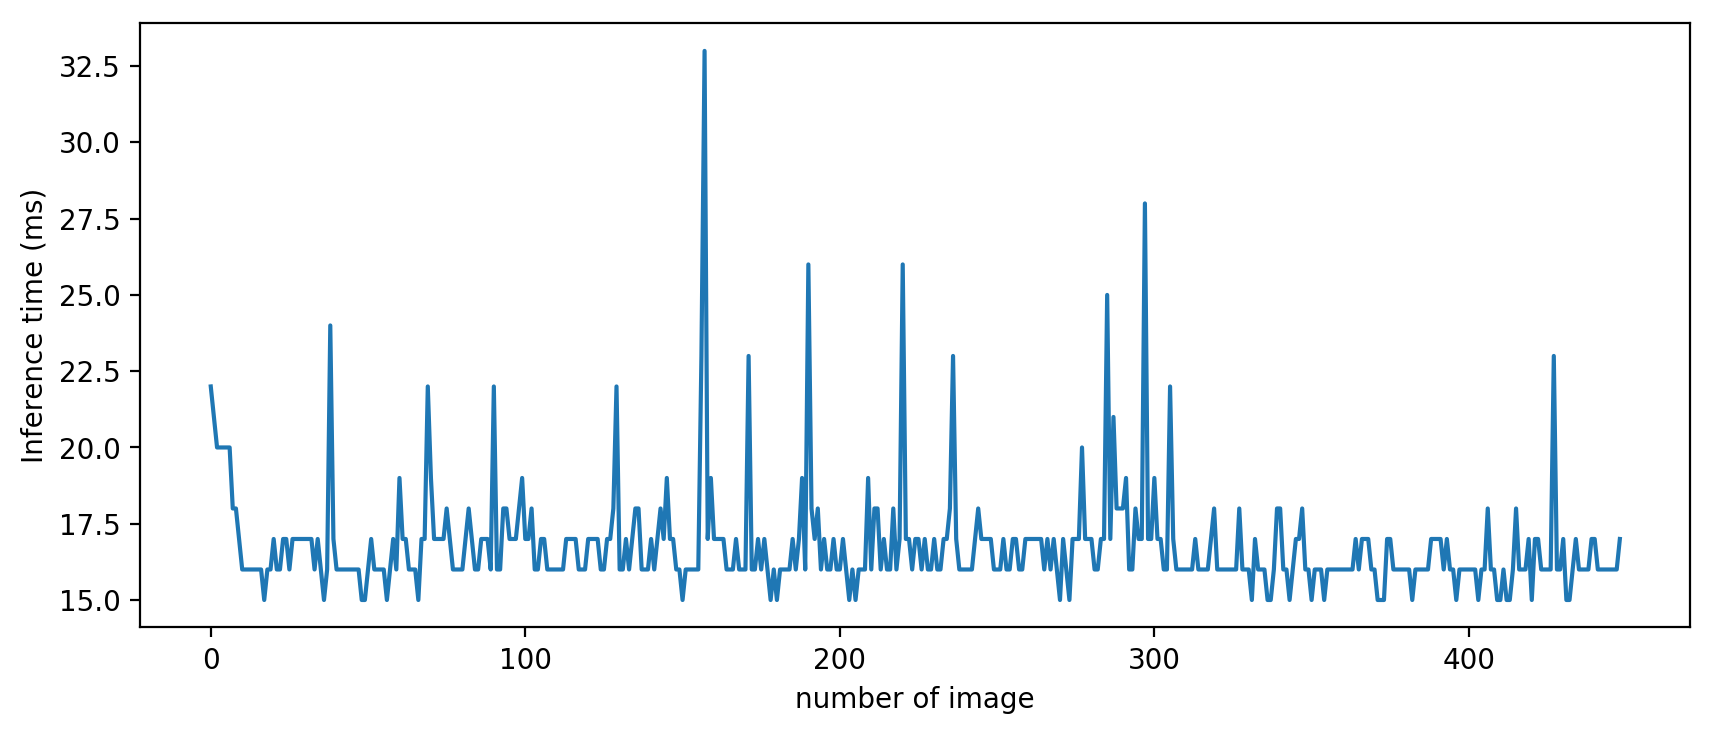
\includegraphics[width=15cm]{figures/Inftime_yolov5L_half.png}
    \caption{The inference time of YOLOv5l model, when it run on GPU with half precision}
    \label{fig: gpulh}
\end{figure}
\begin{figure}[H]
    \centering
    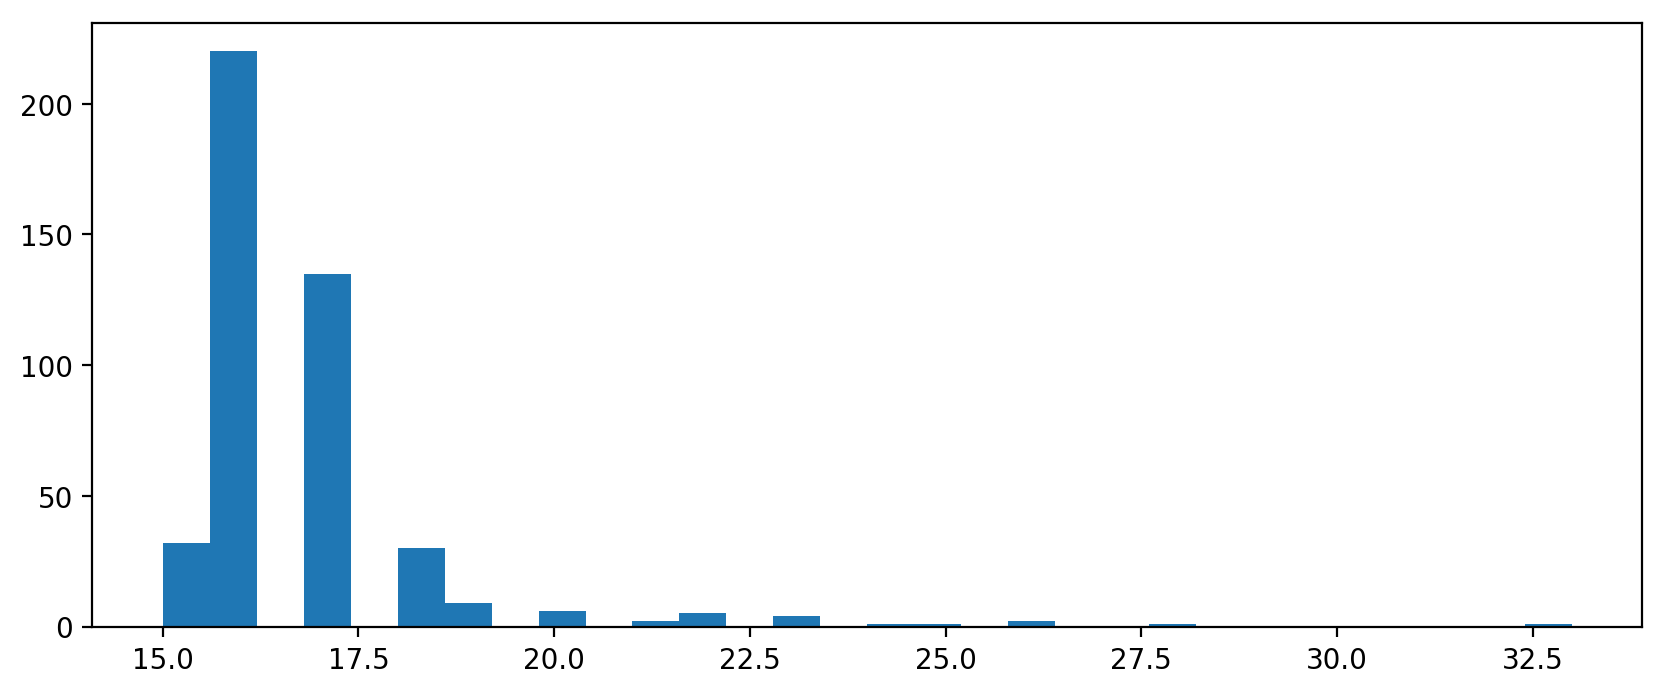
\includegraphics[width=15cm]{figures/Inftime_yolov5L_half_hist.png}
    \caption{The histogram of inference time of YOLOv5l model, when it run on GPU with half precision}
    \label{fig: gpulh_hist}
\end{figure}
% Here the inference time of Yolov5s model on 470 images of kaggle data set, with half precision is shown in Fig. \ref{fig: gpus_half}. Fig. \ref{fig: gpus_half_hist} shows the histogram of these recorded time.
% \begin{figure}[H]
%     \centering
%     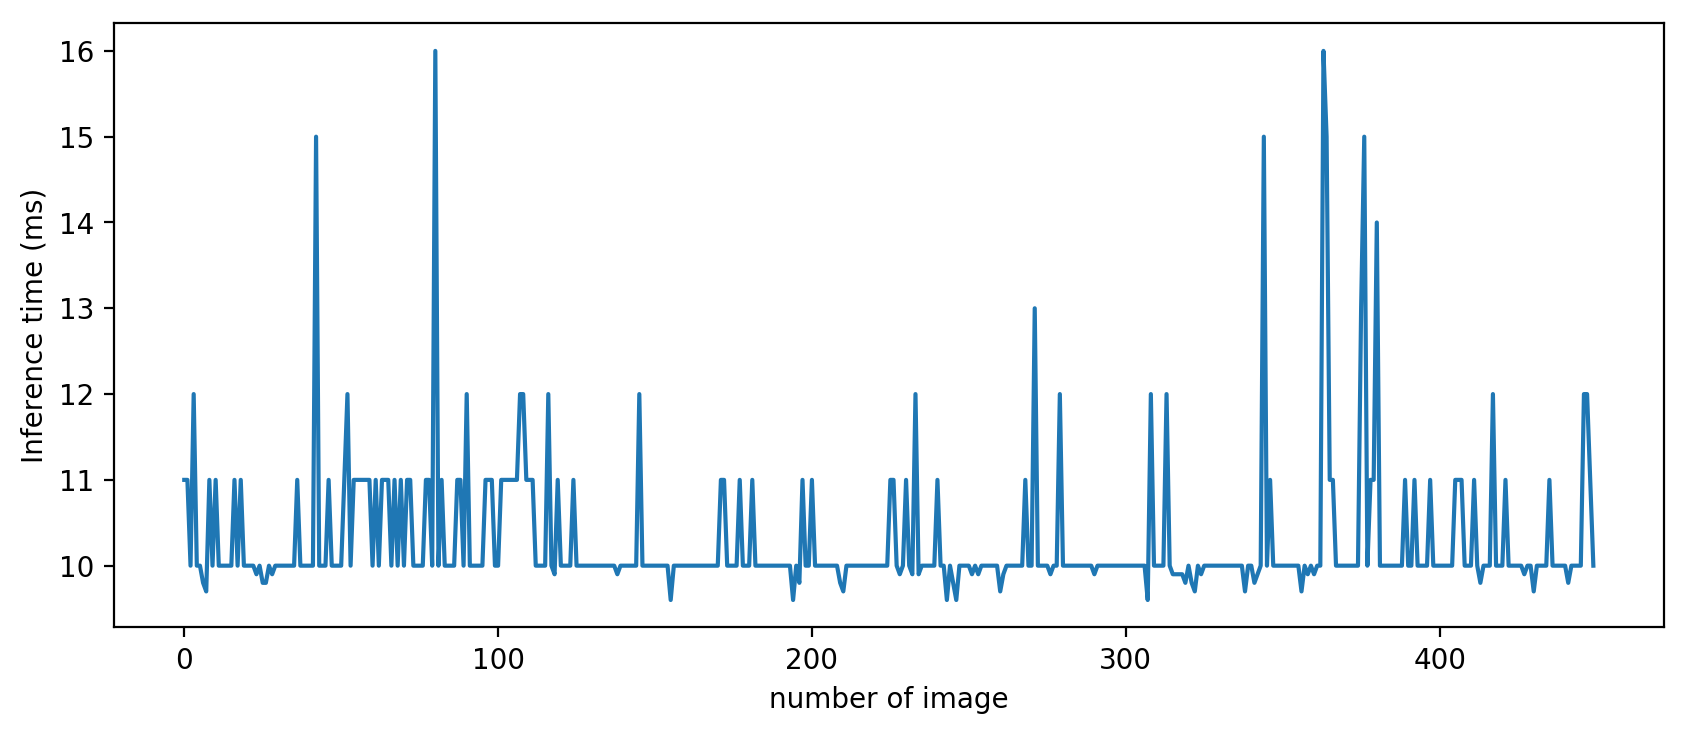
\includegraphics[width=15cm]{figures/Inftime_yolov5s_half.png}
%     \caption{The inference time of YOLOv5s model with half precision, when it run on GPU}
%     \label{fig: gpus_half}
% \end{figure}
% \begin{figure}[H]
%     \centering
%     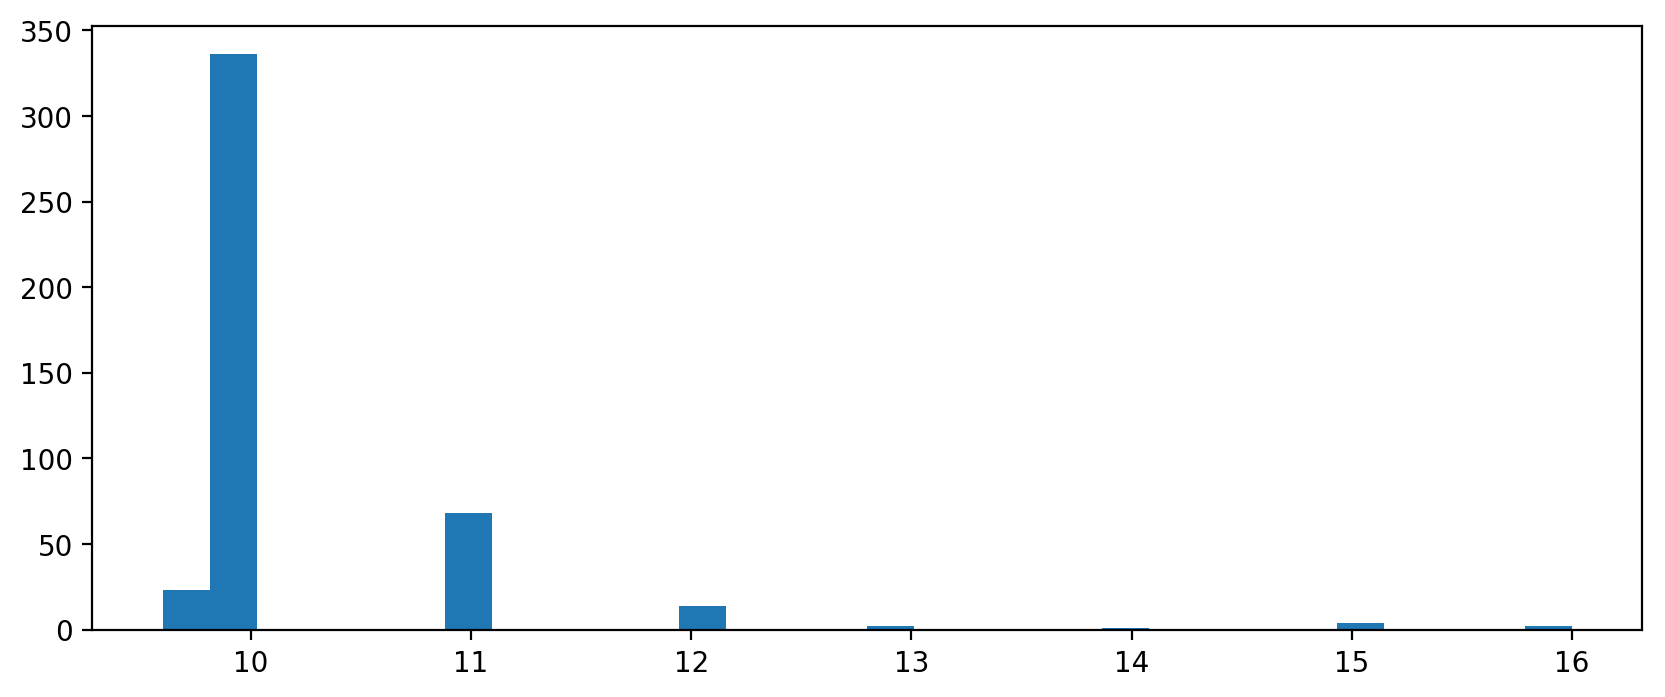
\includegraphics[width=15cm]{figures/Inftime_yolov5s_half_hist.png}
%     \caption{The histogram of inference time of YOLOv5s model with half precision, when it run on GPU}
%     \label{fig: gpus_half_hist}
% \end{figure}
% % \subsubsection*{GPU pro}
The maximum inference time is equal to 33.0 (ms). The minimum inference time is 15.0 (ms) and the standard deviation is 1.76. The total time is 7.532 (s).

%%%%%%%%%%%%%%% NEW SECTION %%%%%%%%%%%%%%%
\subsection*{Inference time of CPU}
Here you can find the inference time of Yolov5l model on 470 images of kaggle data set, which selected as a test set in Fig. \ref{fig: cpul}. Fig. \ref{fig: cpul_hist} shows the histogram of these time.
\begin{figure}[H]
    \centering
    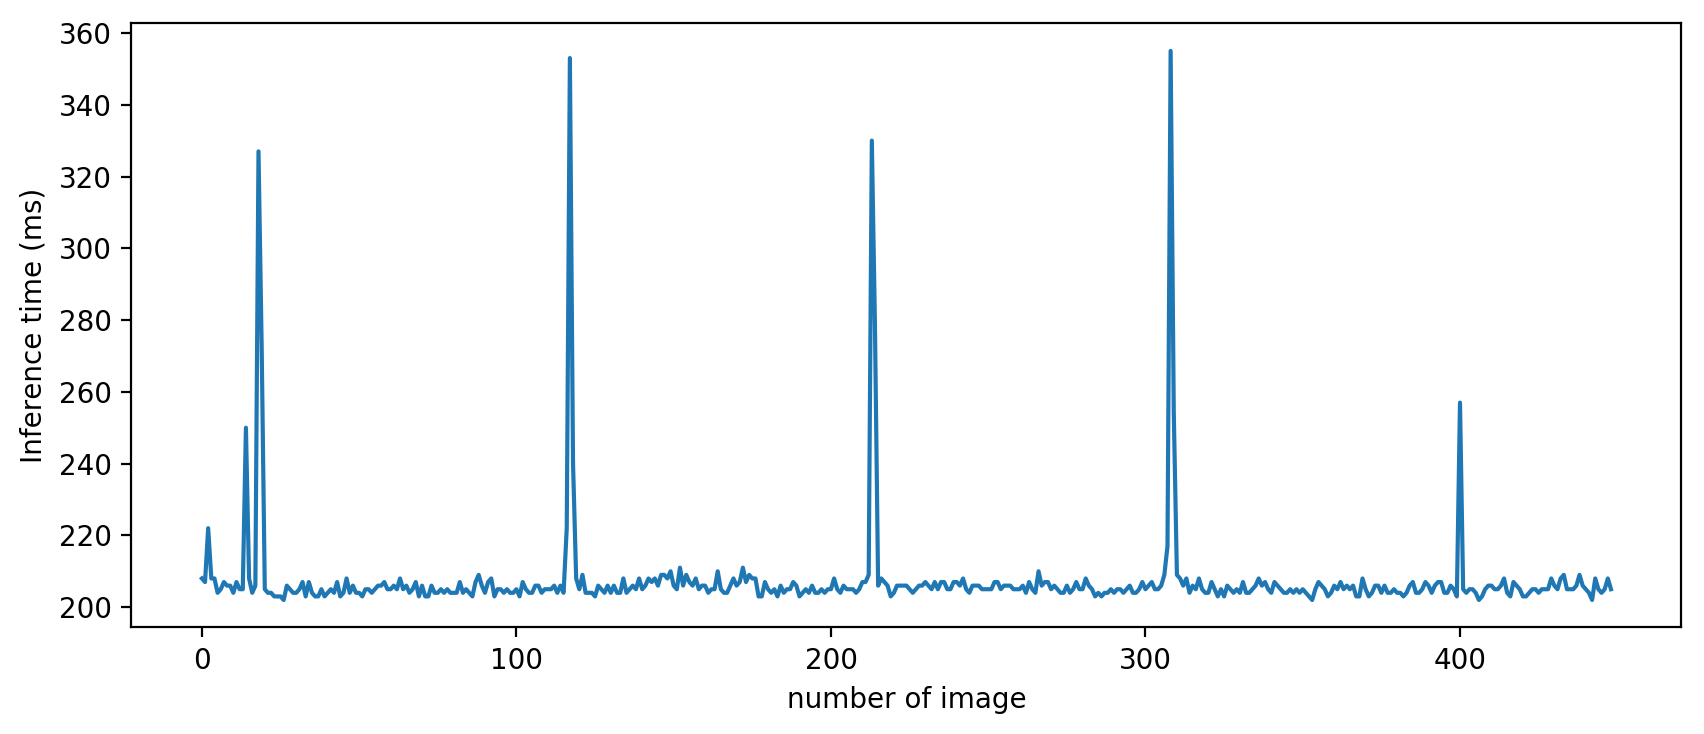
\includegraphics[width=15cm]{figures/Inftime_yolov5L_cpu.png}
    \caption{The inference time of YOLOv5l model, when it run on CPU}
    \label{fig: cpul}
\end{figure}
\begin{figure}[H]
    \centering
    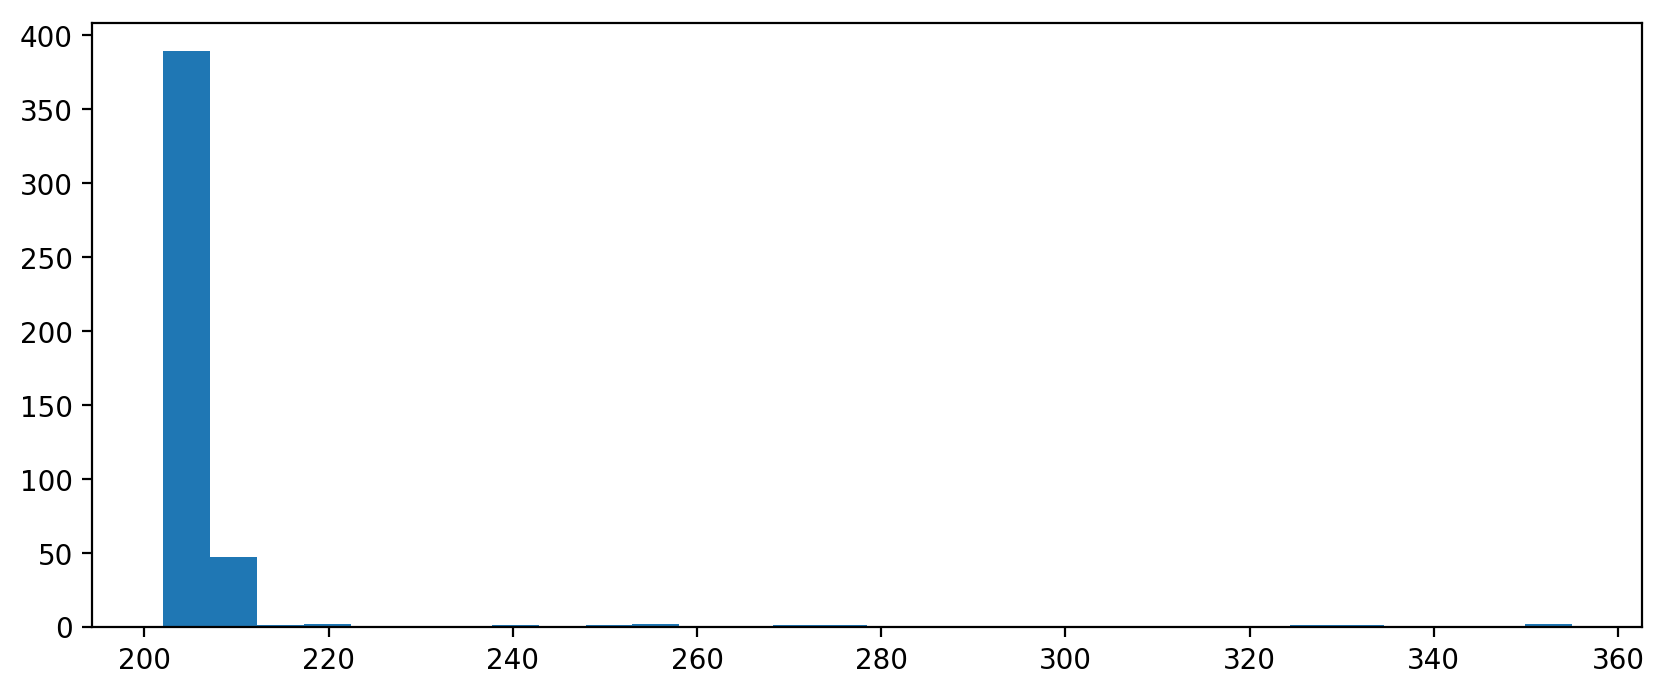
\includegraphics[width=15cm]{figures/Inftime_yolov5L_cpu_hist.png}
    \caption{The histogram of inference time of YOLOv5l model, when it run on CPU}
    \label{fig: cpul_hist}
\end{figure}
The maximum inference time is equal to 355.0 (ms). The minimum inference time is 202.0 (ms) and the standard deviation is 14.36. The total time is 93.110 (s).

%%%%%%%%%%%%%%% NEW SECTION %%%%%%%%%%%%%%%
\section*{Compare the results}

\begin{table}[H]
    \caption{The inference time with different scenarios for YOLOv5s model}
    \label{tab: Data}
    \centering
    \begin{tabular}{c|c|c|c|c|c}
    \toprule
     \textbf{Name} &\bf{Min (ms)}& \bf{Max (ms)} & \textbf{Average (ms)}  & \textbf{Std} & \textbf{Total time (s)} \\
     \midrule
     GPU & 7.8 & 16 & 9.4 & 1.42 & 4.23\\
     GPU-half & 9.6 & 16 & 10.29 & 0.81 & 4.63 \\
     CPU & 375 & 726 & 396.12 & 34.82 & 178.255  \\
     \bottomrule
    \end{tabular}
\end{table}
\begin{table}[H]
    \caption{The inference time with different scenarios for YOLOv5m model}
    \label{tab: Data}
    \centering
    \begin{tabular}{c|c|c|c|c|c}
    \toprule
     \textbf{Name} &\bf{Min (ms)}& \bf{Max (ms)} & \textbf{Average (ms)} & \textbf{Std} & \textbf{Total time (s)} \\
     \midrule
     GPU & 13 & 28 & 13.49 & 1.37 & 6.127\\
     GPU-half & 11 & 21 & 12.75 & 1.21 & 5.788 \\
     CPU & 100 & 999 & 143.85 & 187.73 & 65.311  \\
     \bottomrule
    \end{tabular}
\end{table}

\begin{table}[H]
    \caption{The inference time with different scenarios for YOLOv5l model}
    \label{tab: Data}
    \centering
    \begin{tabular}{c|c|c|c|c|c}
    \toprule
     \textbf{Name} &\bf{Min (ms)}& \bf{Max (ms)} & \textbf{Average (ms)} & \textbf{Std} & \textbf{Total time (s)}  \\
     \midrule
     GPU & 24 & 52 & 27.17 & 1.96 & 12.201\\
     GPU-half & 15 & 33 & 16.77 & 1.76 & 7.532 \\
     CPU & 202 & 355 & 207.37 & 14.36 & 93.11  \\
     \bottomrule
    \end{tabular}
\end{table}
% %%%%%%%%%%%%%%% NEW SECTION %%%%%%%%%%%%%%%
% \section*{Problem 3: How to include graphics?}
% Images, figures, and photos are usually included in the context using the command \texttt{includegraphics}  inside \texttt{figure} environment.

% \begin{verbatim}
%     \begin{figure}[H]
%         \centering
%         \includegraphics[options]{filename}
%         \caption{caption for the figure}
%         \label{fig: figlabel}
%     \end{figure}
% \end{verbatim}

% Figure \ref{fig: ElemntsPE} shows some elements that are frequently used in power electronic converters. This figure is adopted from \cite{FPE}.

% \begin{figure}[H]
%     \centering
%     \includegraphics[width=15cm]{figures/elements.png}
%     \caption{Elements of power electronic converters}
%     \label{fig: ElemntsPE}
% \end{figure}

% For more information on how to use this package, please visit the following website: \\
% \url{https://latexref.xyz/_005cincludegraphics.html}



% %%%%%%%%%%%%%%% NEW SECTION %%%%%%%%%%%%%%%
% \section{Problem 4: How to cite?}
% Paper \cite{Gole97} provides guidelines for modeling power electronics in electric power engineering application. If you do not include any reference please delete the reference section at the end of the document (see three lines of code before \texttt{\textbackslash end\{document\}})









% %%%%%%%%%%%%%%% REFERENCES %%%%%%%%%%%%%%%
% \newpage
% \bibliographystyle{IEEEtran}
% \bibliography{References}








\end{document}
